% !TEX TS-program = pdflatex
\documentclass[12pt,a4paper]{article}

% ====== Packages ======
\usepackage[margin=2.5cm]{geometry}
\usepackage{setspace}
\usepackage{graphicx}
\usepackage{array}
\usepackage{booktabs}
\usepackage{threeparttable}
\usepackage{subcaption}
\usepackage{amsmath,amssymb,amsfonts}
\usepackage{siunitx}
\usepackage{caption}
\usepackage{enumitem}
\usepackage{longtable}
\usepackage{float}
\usepackage{multirow}
\usepackage{xcolor}
\usepackage[authoryear]{natbib}
\usepackage{tocloft}
\usepackage{authblk}
\usepackage{hyperref}

\graphicspath{{figures/}}

% ====== Formatting ======
\onehalfspacing
\setlist[itemize]{leftmargin=*, itemsep=2pt, topsep=2pt}
\setlist[enumerate]{leftmargin=*, itemsep=2pt, topsep=2pt}
\hypersetup{colorlinks=true, linkcolor=black, citecolor=black, urlcolor=blue}

% ====== Custom commands ======
\newcommand{\DPMO}{\mathrm{DPMO}}
\newcommand{\Cpk}{C_{pk}}
\newcommand{\Recall}{\ensuremath{\mathrm{Recall}}}
\newcommand{\Precision}{\mathrm{Precision}}
\newcommand{\Fone}{\mathrm{F1}}
\newcommand{\AUC}{\ensuremath{\mathrm{AUC}}}
\newcommand{\Accuracy}{\mathrm{Accuracy}}
\newcommand{\Sig}{\sigma}
\newcommand{\tighttabcolsep}{\setlength{\tabcolsep}{4.5pt}}

% ====== Title block ======
\title{\textbf{Automated Quality Control in Aquaculture: A Six Sigma Approach to Salmon Disease Detection using Convolutional Neural Networks}\\[6pt]
{\large IND310 Report}}
\author[1]{Gabriel Temitayo Fayomi}
\author[1]{Mads Teien}
\affil[1]{Norwegian University of Life Sciences, REALTEK, Industrial Economics (INDØK)}
\date{\today}

\begin{document}
\maketitle

\begin{abstract}
This study analyzes automated image-based disease detection in Atlantic salmon as an Operations Research problem that integrates supervised classification with statistical quality control and capability analysis in aquaculture. The objective is to evaluate whether convolutional neural networks (CNNs) for \emph{Fresh} versus \emph{Infected} identification can deliver process capability suitable for pen-level decision support. We conduct a modelling study on the public \emph{SalmonScan} dataset, training three baseline CNN architectures and a soft-voting ensemble. Performance is estimated using a multi-seed validation strategy (10 train-test splits) to obtain robust mean metrics and uncertainty estimates. Results are translated into Six Sigma indicators including DPMO and Sigma levels. The ensemble achieved a mean Recall of 97.7\% for infected fish detection, corresponding to approximately a 3.5$\sigma$ process capability level. Notably, the three individual CNN architectures showed no statistically significant differences in mean performance, while the ensemble provided measurable improvement through variance reduction. We discuss significant caveats regarding overfitting and domain shift. The contribution is a transparent bridge from machine learning metrics to capability indices that operations managers already use, enabling control-chart monitoring.
\end{abstract}

\section{Business Understanding}

\subsection{Background \& Context}
The Norwegian Atlantic salmon farming industry represents a cornerstone of the national economy and a critical component of the global food supply chain. However, the industry's growth is currently constrained by a "biological ceiling," primarily defined by challenges related to fish health and welfare. In 2024, the sector reported significant losses, with the Norwegian Veterinary Institute documenting that 45.8 million salmon died in land-based hatcheries and another 57.8 million died during the sea phase \citep{NVI_2025_NFHR2024}. These mortality rates, often exceeding 15\% in the sea phase, represent not only an animal welfare crisis but also a substantial economic inefficiency.

Disease outbreaks, such as Pancreas Disease (PD), Infectious Salmon Anemia (ISA), and complications arising from sea lice infestations, are major drivers of these losses. \cite{AUNSMO2010233} developed stochastic models illustrating the direct costs of diseases like PD, highlighting how mortality, reduced growth, and carcass downgrading impact profitability. Furthermore, \cite{IVERSEN2020735089} analyzed production costs across major salmon farming nations, identifying biological challenges as the primary differentiator in competitiveness. As feed and lice treatment costs continue to rise \citep{Iversen2017}, the economic imperative to detect and mitigate disease early has never been stronger.

To address these challenges, the industry is increasingly adopting "Precision Fish Farming" (PFF). Defined by \cite{FORE2018176}, PFF applies control-engineering principles to aquaculture, moving management from experience-based decisions to data-driven operations. By utilizing sensors, cameras, and automated analysis, PFF aims to monitor the animal continuously without the stress associated with physical handling. This project aligns directly with the PFF framework, leveraging computer vision to automate the detection of health indicators.

\subsection{The Current "As-Is" Process}
To understand the necessity of an automated solution, one must first analyze the limitations of the current manual inspection regime. The standard procedure for health monitoring in Norwegian aquaculture is a labor-intensive and stressful event for the biomass.

Typically, a health inspection involves the following steps \citep{NVI_2025_NFHR2024}:
\begin{enumerate}
    \item \textbf{Starvation:} The fish are starved for 24 hours prior to handling to reduce metabolic rate and waste production.
    \item \textbf{Crowding:} The net pen is raised, or a sweep net is used to crowd the fish into a smaller volume, increasing density and stress.
    \item \textbf{Extraction:} A sample of fish (often as few as 10-20 individuals from a population of 100,000) is pumped onto a service vessel or scooped out with a dip net.
    \item \textbf{Anesthesia:} To allow for close inspection, the fish are often anesthetized in a tank.
    \item \textbf{Manual Inspection:} A fish health biologist or veterinarian visually inspects the fish for external signs of disease (lice, ulcers, deformities) and may perform autopsies on moribund fish.
    \item \textbf{Release:} Surviving fish are returned to the pen.
\end{enumerate}

This "As-Is" process suffers from two critical flaws. First, the \textbf{sampling error} is massive; inspecting 20 fish out of 100,000 provides a statistically insignificant snapshot of the population health (0.02\% sample rate) \citep{montgomery2020introduction}. Second, the \textbf{handling stress} itself can induce disease outbreaks \citep{Iversen2017}. The physical abrasion removes the protective mucus layer, making the fish susceptible to secondary bacterial infections, while the stress hormones (cortisol) suppress the immune system \citep{Deng2025}. Thus, the act of measuring the quality of the process actually degrades the quality of the product.

\subsection{Economic Impact Analysis}
The financial justification for an automated early-warning system can be illustrated through a hypothetical "Cost of Poor Quality" (COPQ) calculation. Consider a single standard net pen containing 100,000 Atlantic salmon with an average weight of 4.0 kg. At a market price of 80 NOK/kg, the standing biomass value is:
\begin{equation}
    \text{Value} = 100,000 \text{ fish} \times 4.0 \text{ kg/fish} \times 80 \text{ NOK/kg} = \mathbf{32,000,000 \text{ NOK}}
\end{equation}

Let us compare two scenarios following a Pancreas Disease (PD) infection:

\textbf{Scenario A: Late Detection (Current State)}
Without continuous monitoring, the disease spreads unnoticed until mortality spikes.
\begin{itemize}
    \item \textbf{Mortality:} 20\% of the stock dies (20,000 fish).
    \item \textbf{Downgrading:} The surviving fish suffer from reduced growth and quality. 50\% of survivors are downgraded from "Superior" to "Production" grade, losing 20 NOK/kg in value.
    \item \textbf{Direct Loss:}
    \begin{itemize}
        \item Mortality Cost: $20,000 \times 4 \times 80 = 6,400,000$ NOK
        \item Quality Loss: $40,000 \times 4 \times 20 = 3,200,000$ NOK
        \item \textbf{Total COPQ:} \textbf{9,600,000 NOK}
    \end{itemize}
\end{itemize}

\textbf{Scenario B: Early Detection (Future State)}
The AI system detects the first signs of skin lesions or behavioral changes.
\begin{itemize}
    \item \textbf{Action:} Immediate harvesting of the infected pen or targeted treatment.
    \item \textbf{Outcome:} Mortality is capped at 2\%. No quality downgrading for the majority of the stock.
    \item \textbf{Direct Loss:} $2,000 \times 4 \times 80 = 640,000$ NOK.
\end{itemize}

In this simplified model, the \textbf{Value of Information} provided by the AI system is approximately \textbf{8.96 Million NOK per pen per cycle}. Even if the system is only 50\% effective, the ROI remains substantial, justifying the investment in "Quality 4.0" technologies \citep{Tsung2023, 10.1108/TQM-11-2023-0361}.

\subsection{Deployment Concept Overview}
Translating the modelling results into an operational solution requires a realistic deployment concept that fits within existing farm infrastructure. Following the Precision Fish Farming framework \citep{FORE2018176}, the envisioned system consists of three main layers: (1) a sensing layer with underwater cameras, (2) an edge computing layer for on-site inference, and (3) an integration layer connecting to farm management systems. From a Six Sigma perspective, this architecture embeds the "Measure" and "Analyze" phases of DMAIC directly into the production process \citep{Tsung2023, montgomery2020introduction}. Detailed system architecture and hardware considerations are presented in Section~\ref{sec:deployment}.

\subsection{Human-in-the-Loop Workflow}
Despite high model performance, full automation of health decisions would be neither acceptable nor responsible. Instead, the proposed system implements a "human-in-the-loop" workflow, aligning with recent Quality 4.0 recommendations \citep{10.1108/TQM-11-2023-0361}. The AI system acts as a first-line filter that flags potential infections for expert review, rather than making autonomous treatment decisions. This "screen-and-refer" approach mitigates automation bias while leveraging the CNN's ability to pre-screen tens of thousands of fish images that would otherwise go unseen. The detailed workflow is described in Section~\ref{sec:deployment}.

\subsection{Operational Risks and Change Management}
Introducing AI-driven quality control into an established production system entails organizational as well as technical risks. Drawing on lessons from Lean Six Sigma implementations in healthcare \citep{Henrique17022020} and Integrated Quality 4.0 frameworks \citep{10.1108/TQM-11-2023-0361}, several factors are critical:
\begin{itemize}
    \item \textbf{Stakeholder Acceptance:} Farm managers and veterinarians must trust that the system adds value rather than undermining their expertise. Transparent performance metrics, explainable visualizations, and pilot projects with clear success criteria can help build this trust.
    \item \textbf{Standardization:} To reduce domain shift and Clever Hans effects, farms may need to standardize camera placement, background panels, and illumination conditions. While this requires upfront effort, it aligns with broader Quality Management principles of process standardization \citep{montgomery2020introduction}.
    \item \textbf{Training and SOPs:} Staff must be trained not only on the technical interface but also on how to interpret probabilities and confidence intervals. Clear SOPs should specify when an alert mandates physical sampling, quarantine measures, or other interventions.
    \item \textbf{Data Governance:} As more image and sensor data are collected, questions arise about data ownership, sharing, and privacy. Although images of fish do not raise the same ethical issues as human medical data, commercial sensitivities remain. Contracts between technology providers and farmers should address who owns derived models and data streams \citep{BIAZI2023102360}.
\end{itemize}

Handled properly, these challenges are surmountable and largely mirror those observed when introducing electronic health records and decision-support systems in hospitals. The key is to treat the AI system as a socio-technical intervention rather than a purely technical upgrade.

\subsection{Problem Statement}
Current disease detection methods largely rely on manual inspection, which is labor-intensive, subjective, and inherently reactive. Inspections often occur only after mortality rates spike or during stressful handling events like lice counting. This delay allows pathogens to spread within a pen before countermeasures are enacted. Furthermore, manual checks are prone to human error and fatigue, and the physical handling of fish can damage their mucus layer, making them more susceptible to secondary infections.

From an Operations Research and Quality Control (QC) perspective, we frame this as a defect detection process. Here, a ``unit'' is an individual salmon, and a ``defect'' is the presence of visible disease symptoms. The operational problem is to design a non-invasive ``early warning'' system that can screen the population and flag potential ``defects'' for human intervention.

\subsubsection{Research Questions}
To guide this study and ensure methodological coherence, we formulate one overarching research question with three supporting sub-questions:

\textbf{Main Research Question:}
\begin{quote}
\emph{To what extent can convolutional neural networks provide process capability suitable for pen-level disease screening in Atlantic salmon aquaculture, and how can their performance be translated into actionable quality control metrics for operations managers?}
\end{quote}

This main question is operationalized through the following sub-questions:

\begin{enumerate}
    \item \textbf{RQ1 (Model Performance):} What classification accuracy, recall, and precision can CNN architectures achieve for binary (Fresh vs.\ Infected) salmon disease detection on the SalmonScan dataset, and do deeper architectures provide statistically significant improvements over shallow ones?
    
    \item \textbf{RQ2 (Quality Metrics Translation):} How can standard machine learning performance metrics (Recall, Precision, F1-Score) be meaningfully translated into Six Sigma process capability indicators (DPMO, Sigma level) to support operational decision-making in aquaculture?
    
    \item \textbf{RQ3 (Deployment Viability):} What are the primary technical and organizational barriers to deploying CNN-based disease detection in real-world sea pen environments, and what mitigation strategies can address domain shift between laboratory and operational conditions?
\end{enumerate}

\subsection{Project Objectives}
The primary objective of this study is to develop and evaluate a Convolutional Neural Network (CNN) capable of performing binary classification (\emph{Fresh} vs. \emph{Infected}) on images of Atlantic salmon. This model is not intended to replace veterinary diagnosis but to support a "screen-and-refer" decision workflow. In this workflow, the AI acts as a first-line filter, processing large volumes of image data to identify high-risk individuals for expert review.

The specific objectives are:
\begin{enumerate}
    \item \textbf{Maximize Recall (Sensitivity):} The cost of a False Negative (missing an infected fish) is extremely high, as it allows disease to propagate. Therefore, the model must prioritize detecting "Infected" cases, even at the expense of some False Positives.
    \item \textbf{Maintain Acceptable Precision:} While Recall is paramount, Precision must remain high enough to prevent "alert fatigue" among operators. A system that flags too many healthy fish as sick will eventually be ignored.
    \item \textbf{Quantify Process Capability:} We aim to translate standard Machine Learning metrics into Six Sigma indicators (Sigma Level, DPMO) to provide operations managers with a clear measure of the system's reliability in a production context.
\end{enumerate}

\subsection{Success Criteria}
To determine if the model is "fit-for-use," we define success through a combination of Machine Learning performance and Six Sigma quality standards:
\begin{itemize}
    \item \textbf{ML Metrics:} The model should achieve a Recall of $\ge$ 95\% and an F1-Score of $\ge$ 95\% on the test set.
    \item \textbf{Six Sigma Metrics:} The process should achieve a Sigma Level of $\ge$ 3.0 for the "Infected" class, with 4$\sigma$ representing a stretch goal. In Six Sigma theory, a 3$\sigma$ process (93.3\% yield) is considered the minimum acceptable threshold, while 4$\sigma$ indicates a stable, production-ready system \citep{Tsung2023}.
    \item \textbf{Operational Viability:} The solution must demonstrate the potential for deployment in a pen-level monitoring workflow, offering a tangible improvement over random sampling.
\end{itemize}

\section{Literature Review}

The intersection of aquaculture, computer vision, and quality management represents a rapidly evolving interdisciplinary field. This review synthesizes literature from three distinct domains: deep learning architectures for object detection, specific challenges in underwater imaging, and the integration of artificial intelligence into statistical quality control frameworks (Quality 4.0).

\subsection{Deep Learning Architectures in Aquaculture}
The application of Computer Vision (CV) in aquaculture has shifted significantly from traditional image processing to Deep Learning (DL) in recent years. \cite{Pauzi_2021} reviewed the technical workflow for fish disease detection, noting that while early methods relied on handcrafted features (e.g., edge detection, color histograms) and classifiers like Support Vector Machines (SVM), they often struggled with the complex visual variability of biological subjects. \cite{AHMED20225170} compared SVMs with early neural networks, demonstrating that while SVMs are computationally efficient, they lack the feature abstraction capabilities required for robust disease identification in uncontrolled environments.

Modern approaches predominantly utilize Convolutional Neural Networks (CNNs). \cite{HaddadMohammed2025} and \cite{AlZubi2024} highlight the efficacy of standard architectures such as VGG, ResNet, and Inception for precision fish farming. These models learn hierarchical feature representations, detecting simple edges in early layers and complex pathological patterns (e.g., ulcers, lice) in deeper layers \citep{CHEN2025109507}. \cite{Hasan2022} further validated the use of CNNs for classifying multiple fish diseases, achieving high accuracy on limited datasets.

More recent research has focused on enhancing these backbone architectures. \cite{10138194} proposed a multi-layer fusion network incorporating Attention Mechanisms (specifically the Convolutional Block Attention Module, CBAM). Attention mechanisms allow the network to "focus" on relevant regions of the image (e.g., the lesion) while suppressing background noise, a critical capability for processing underwater images where the background can be cluttered. \cite{BIAZI2023102360} reviewed Industry 4.0 applications in aquaculture, noting that while detection algorithms are maturing, their deployment on edge devices for real-time monitoring remains a significant engineering challenge.

\subsection{Challenges in Underwater Imaging}
Deploying vision models in the marine environment introduces unique challenges not present in terrestrial computer vision. \cite{10048777} and \cite{JIAN2021116088} provide comprehensive reviews of underwater image processing, identifying three primary degradation factors:
\begin{itemize}
    \item \textbf{Light Attenuation:} Water absorbs light at different rates depending on wavelength; red light is absorbed first, leading to the characteristic blue-green cast of underwater imagery.
    \item \textbf{Scattering:} Suspended particles cause light to scatter, resulting in low contrast and haze.
    \item \textbf{Turbidity:} High density of particulate matter can occlude the subject entirely.
\end{itemize}

These factors create a "domain shift" problem. A model trained on high-quality, air-captured images (like the \emph{SalmonScan} dataset) will likely fail when applied to raw underwater footage. \cite{karthika2024deep} suggested multi-modal approaches, fusing visual data with environmental sensors (temperature, turbidity) to improve robustness. Furthermore, \cite{10048777} proposed Domain Adaptation techniques, such as Generative Adversarial Networks (GANs), to synthetically transform underwater images to look like "air" images (or vice versa), thereby bridging the gap between training and operational domains.

\subsection{Data Augmentation and Class Imbalance}
A pervasive issue in medical and biological machine learning is the scarcity of high-quality, annotated data. \cite{Shorten2019} and \cite{wang2017effectiveness} surveyed image data augmentation techniques, concluding that geometric transformations (rotation, flipping, scaling) and photometric adjustments (brightness, contrast) are essential for preventing overfitting in small datasets. \cite{MORENOBAREA2020113696} specifically demonstrated that generative augmentation (using GANs or Variational Autoencoders) can significantly boost classification accuracy on small datasets by creating synthetic samples that fill the gaps in the feature space.

Class imbalance is another critical hurdle; healthy fish vastly outnumber sick ones in a well-managed farm. \cite{s23042333} compared validation strategies for imbalanced learning, arguing that standard cross-validation can yield overly optimistic performance estimates. They recommend Distribution-Balanced Stratified Cross-Validation (DOB-SCV) and the use of oversampling techniques like SMOTE (Synthetic Minority Over-sampling Technique) to ensure the model learns to recognize the minority class (diseased fish) effectively.

\subsection{Explainable AI (XAI) and Trust}
As AI systems are integrated into decision-making loops, the "Black Box" nature of Deep Learning becomes a liability. Operators need to know \emph{why} a model flagged a fish as infected. \cite{selvaraju2017gradcamdidsaythat} introduced Gradient-weighted Class Activation Mapping (Grad-CAM), a technique that visualizes the regions of an image that influenced the model's prediction. In the context of disease detection, Grad-CAM should highlight the specific lesion or parasite.

However, \cite{Lapuschkin2019} warned of the "Clever Hans" effect, where models learn spurious correlations (e.g., classifying a fish as "infected" because of a specific background color present only in training images of sick fish). \cite{CHEN2025109507} emphasized that in medical imaging, XAI is not just a "nice-to-have" but a safety requirement to verify that the model is detecting pathology rather than artifacts.

\subsection{Quality 4.0: Integrating AI with Six Sigma}
The integration of Machine Learning with traditional Quality Control methodologies is a core component of "Quality 4.0." \cite{10.1108/TQM-11-2023-0361} proposed an "Integrated Quality 4.0 Framework" that embeds ML techniques directly into the Six Sigma DMAIC (Define, Measure, Analyze, Improve, Control) cycle. They argue that while Six Sigma provides the structured problem-solving approach and statistical rigor \citep{montgomery2020introduction}, ML offers superior analytical power for complex, non-linear variables.

While Six Sigma originated in manufacturing, its application has expanded to biological sectors. \cite{Henrique17022020} reviewed Lean and Six Sigma in healthcare, finding these methodologies effective for reducing medical errors. This is directly analogous to aquaculture, where the "patient" is the fish. By translating biological variability into statistical process capability indices (like Sigma levels), biological risks can be managed with industrial precision \citep{Tsung2023}.

\section{Data Understanding}

\subsection{Dataset Description}
This study utilizes the \emph{SalmonScan} dataset \citep[Version 3]{Ahmed_2024_SalmonScan_V3}, a publicly available collection of images designed for fish disease detection. It is important to note that high-quality, publicly available datasets for aquaculture disease detection are extremely scarce, and the \emph{SalmonScan} dataset is one of the few open-source resources available. The original dataset contains only 24 images of fresh (healthy) fish and 91 images of infected fish. To balance the dataset and increase the sample size, we supplemented the ``Fresh'' class with 26 additional stock images of healthy salmon sourced from iStock, bringing the total to 141 RGB images categorized into two binary classes:
\begin{itemize}
    \item \textbf{Fresh (Healthy):} 50 images representing healthy Atlantic salmon with no visible external symptoms (24 from SalmonScan, 26 from iStock).
    \item \textbf{Infected:} 91 images showing salmon with various visible signs of disease, such as skin lesions, ulcers, discoloration, or fin rot (all from SalmonScan).
\end{itemize}
The supplementary stock images were carefully selected to match the visual style and quality of the original SalmonScan images as closely as possible. Specifically, we chose images with similar backgrounds, lighting conditions, and fish orientations to minimize distributional differences between the original and supplementary samples. While some heterogeneity is unavoidable when combining images from different sources, this curation approach reduces (though does not eliminate) the risk of the model learning source-specific rather than class-specific features. The images are of varying original resolutions and were likely captured using standard digital cameras or smartphones. This scarcity of original data is a primary driver for the methodological choices in this project, particularly the heavy reliance on data augmentation.

\begin{figure}[H]
    \centering
    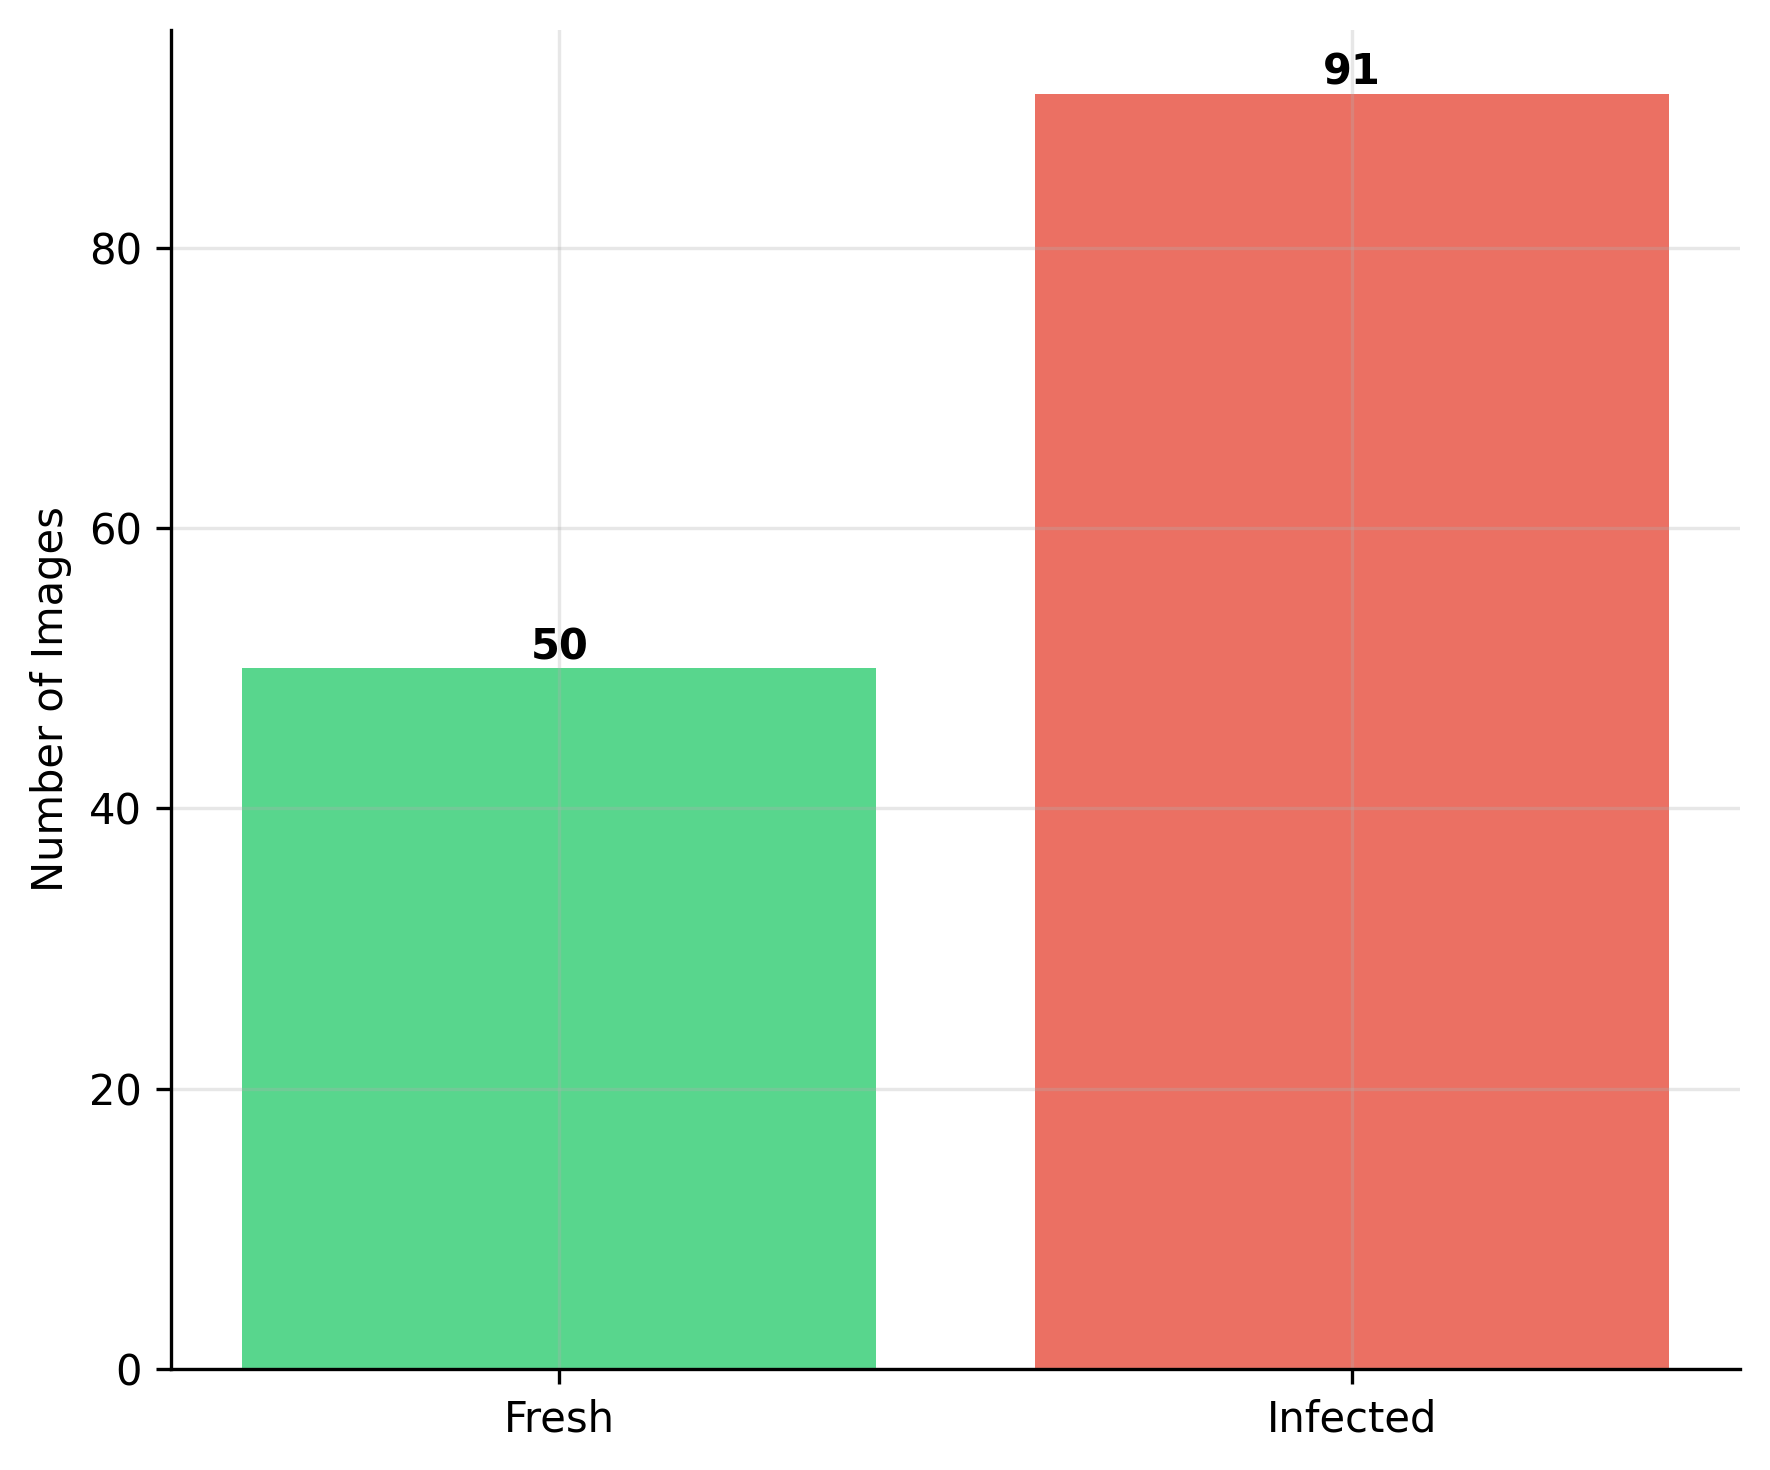
\includegraphics[width=0.9\textwidth]{class_distribution.png}
    \caption{Class distribution in the dataset showing the imbalance between Fresh (50 images) and Infected (91 images) classes.}
    \label{fig:class_distribution}
\end{figure}

\subsection{Exploratory Data Analysis (EDA)}
A thorough understanding of the data is prerequisite to modeling. Our EDA revealed several critical characteristics.

\begin{figure}[H]
    \centering
    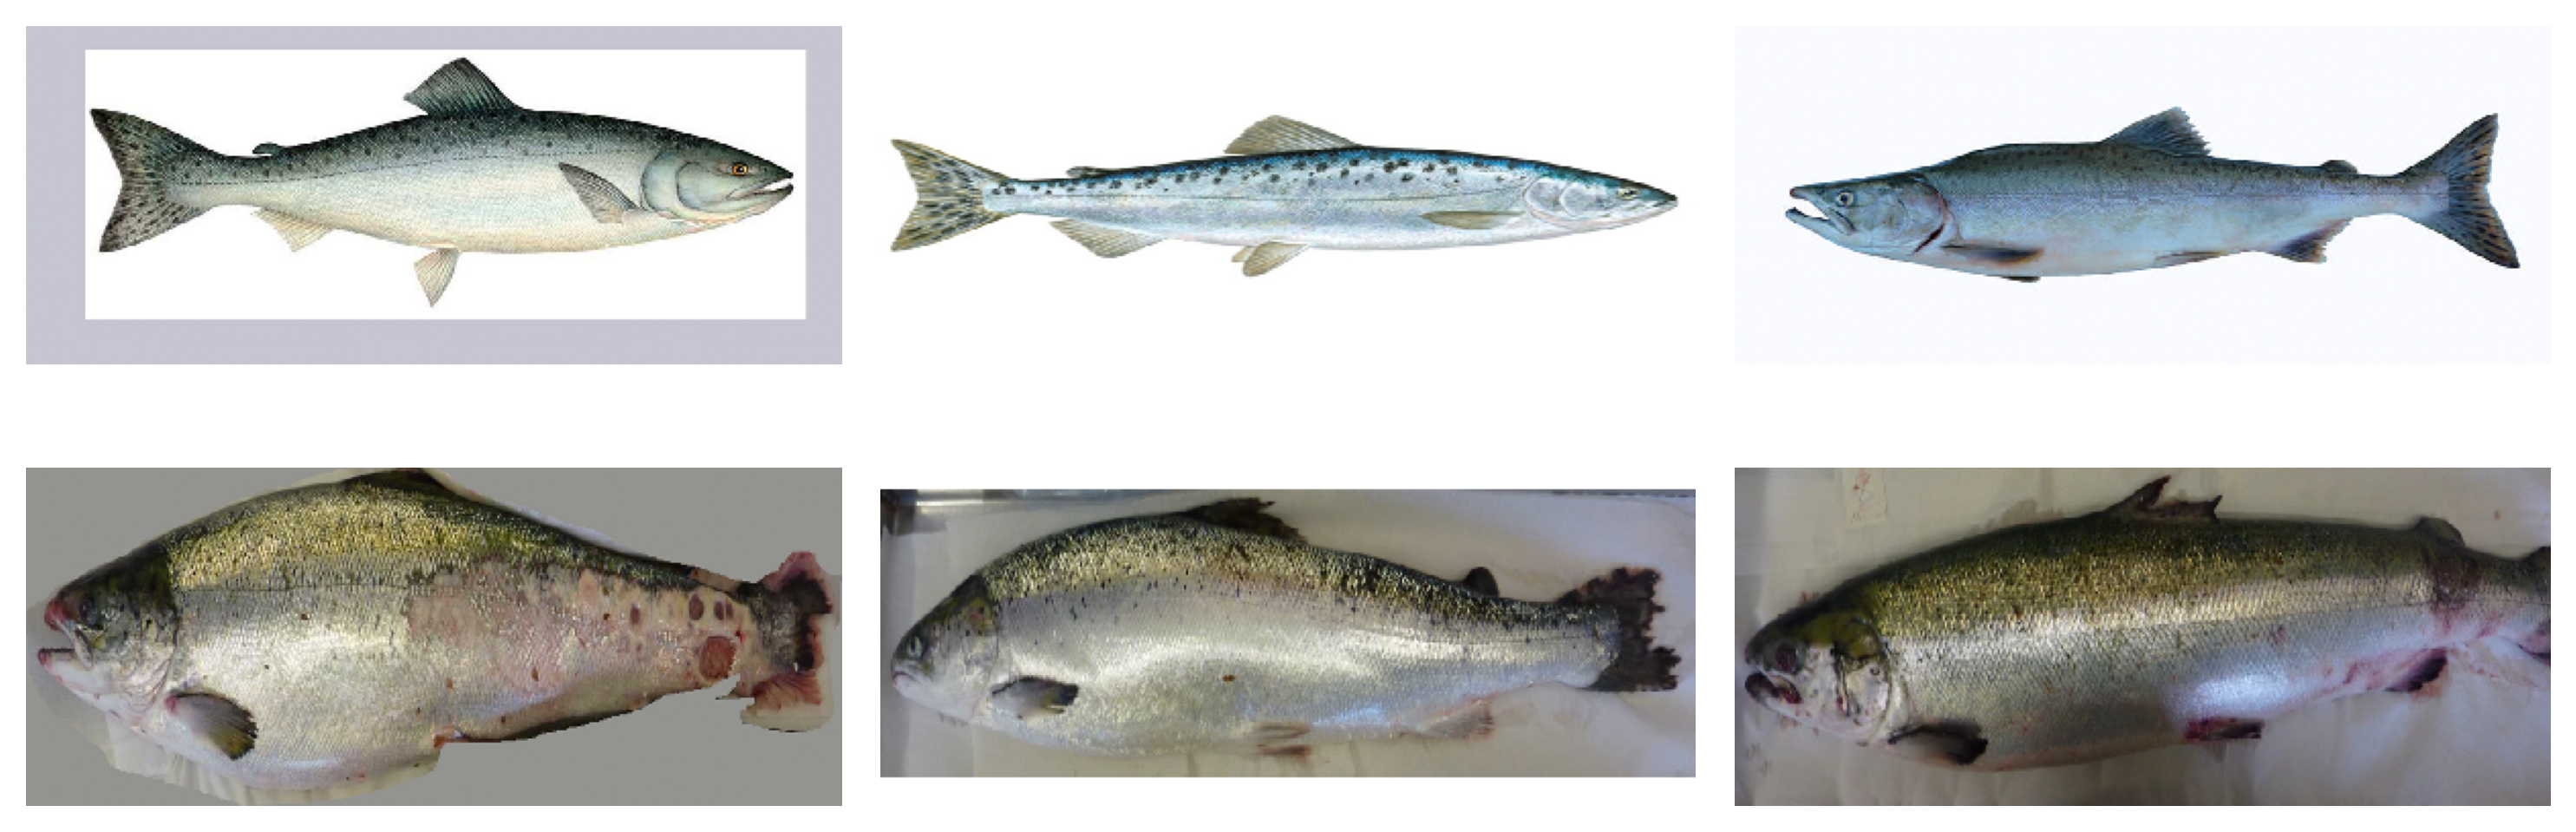
\includegraphics[width=0.95\textwidth]{sample_images.png}
    \caption{Sample images from each class. Top row: Fresh (healthy) salmon. Bottom row: Infected salmon showing visible disease symptoms such as lesions and discoloration.}
    \label{fig:sample_images}
\end{figure}

\textbf{Class Imbalance:} The dataset is imbalanced, with the ``Infected'' class comprising approximately 64\% of the total samples (Figure~\ref{fig:class_distribution}). While this is less severe than the extreme imbalance often found in medical datasets (where positives are rare), it still introduces a bias. A naive model could achieve 64\% accuracy simply by predicting ``Infected'' for every image. We must address this during training, for instance, by using class weights to penalize the misclassification of the minority ``Fresh'' class.

\textbf{Visual Heterogeneity and ``Clever Hans'' Risk:} Visual inspection of the images (Figure~\ref{fig:sample_images}) reveals systematic differences in image processing between the two classes. The fresh fish images (predominantly stock images) feature clean, digitally rendered white backgrounds. In contrast, the infected fish images from SalmonScan have undergone background removal, but this processing is inconsistent---remnants of the original backgrounds (edges, shadows, partial objects) remain visible in many images.
This heterogeneity poses a significant risk known as the ``Clever Hans'' effect \citep{Lapuschkin2019}. Because most ``Fresh'' fish have pristine white backgrounds while ``Infected'' fish often have imperfect background removal artifacts, the CNN might learn to classify based on background cleanliness rather than actual fish pathology. This would lead to a model that performs well on the test set but fails completely in a real-world environment where the background differs from both training conditions.

\subsection{Limitations}
Several limitations inherent to the dataset must be acknowledged:
\begin{itemize}
    \item \textbf{Small Sample Size ($N=141$):} Deep learning models typically require thousands of examples to generalize effectively \citep{BejaniGhatee2021}. With only 141 images, the risk of overfitting---where the model memorizes the training data rather than learning generalizable features---is extremely high \citep{Shorten2019}. This necessitates robust validation strategies such as multi-seed experiments and aggressive data augmentation.
    \item \textbf{Binary Classification Only:} The dataset groups all pathologies into a single "Infected" class. It does not distinguish between specific diseases like PD, ISA, or winter ulcers. Consequently, the model can only serve as a general alert system, not a diagnostic tool.
    \item \textbf{Lack of Metadata:} We lack temporal or geospatial data (e.g., which farm, what time of year). This limits our ability to assess if the model is biased towards specific seasons or locations.
    \item \textbf{Environmental Bias (Domain Shift):} Perhaps the most critical limitation is the "Land vs. Sea" domain shift. The training images appear to be taken "dry" (out of water), likely at a processing plant or during a manual check. However, the target operational environment is underwater in sea pens. Underwater images suffer from light attenuation, scattering, and turbidity \citep{JIAN2021116088}. A model trained on clear, dry images will likely degrade significantly when applied to underwater footage without advanced domain adaptation techniques.
\end{itemize}

\section{Data Preparation}

\begin{figure}[H]
    \centering
    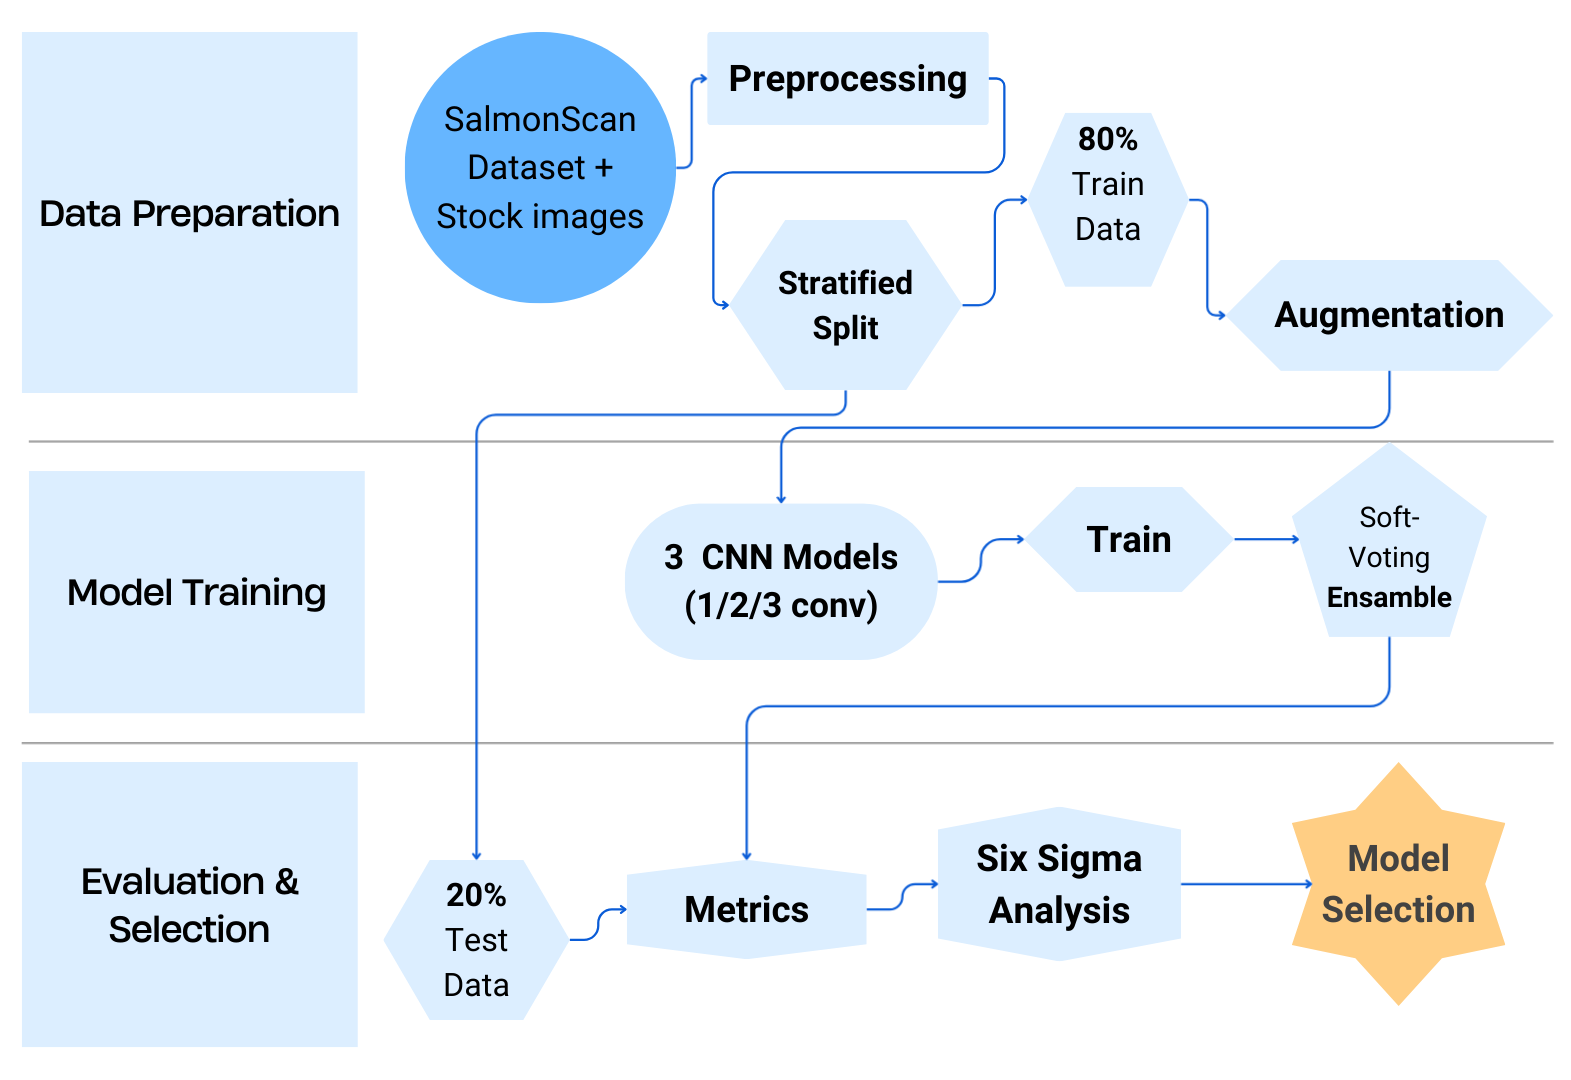
\includegraphics[width=0.95\textwidth]{flow-chart.png}
    \caption{Methodology overview: The complete pipeline from data preparation through model selection. The SalmonScan dataset combined with stock images undergoes preprocessing and stratified splitting (80\% train, 20\% test), with augmentation applied to training data. The entire training process is repeated across 10 random seeds to capture variance from data partitioning and model initialization. Three CNN architectures with varying depths are trained and combined into a soft-voting ensemble. Final model selection is based on metrics evaluated through Six Sigma analysis.}
    \label{fig:methodology_flowchart}
\end{figure}

\subsection{Preprocessing Pipeline}
Data preparation is a critical step in any deep learning pipeline, particularly when dealing with image data. We implemented a standardized preprocessing pipeline to ensure consistency across all inputs.
\begin{itemize}
    \item \textbf{Resizing:} The original images varied significantly in resolution. To create a uniform input tensor for the CNNs, all images were resized to $400 \times 166$ pixels. This specific dimension was chosen to preserve the natural aspect ratio of the salmon (long and slender) while reducing the computational load compared to full-resolution processing.
    \item \textbf{Normalization:} Neural networks converge faster and more stably when input values are small and centered. We normalized the pixel intensity values from the original range of $[0, 255]$ to the range $[0, 1]$ by dividing by 255.
\end{itemize}

\subsection{Data Augmentation}
Given the small dataset size and associated overfitting risk (discussed in Section 3.3), we employed aggressive Data Augmentation \citep{Shorten2019, wang2017effectiveness}. This technique artificially expands the training dataset by creating modified versions of existing images, forcing the model to learn features that are invariant to orientation, position, and scale. We applied the following random transformations:
\begin{itemize}
    \item \textbf{Rotation:} Randomly rotating the image by up to $\pm 15$ degrees.
    \item \textbf{Shifting:} Randomly shifting the image horizontally or vertically by up to 10\%.
    \item \textbf{Shear \& Zoom:} Applying random shear transformations (up to 10\%) and zoom (up to $\pm 10$\%) to simulate different camera angles and distances.
    \item \textbf{Horizontal Flip:} Randomly mirroring the image, as a fish facing left is structurally identical to a fish facing right.
\end{itemize}
Each original training image was augmented 10 times, effectively expanding the training set from approximately 113 samples (80\% of 141) to over 1,100 augmented samples per seed. This 10-fold increase in effective training data is crucial for stabilizing the learning process and achieving the reported performance metrics \citep{MORENOBAREA2020113696, wang2017effectiveness}.

\begin{figure}[H]
    \centering
    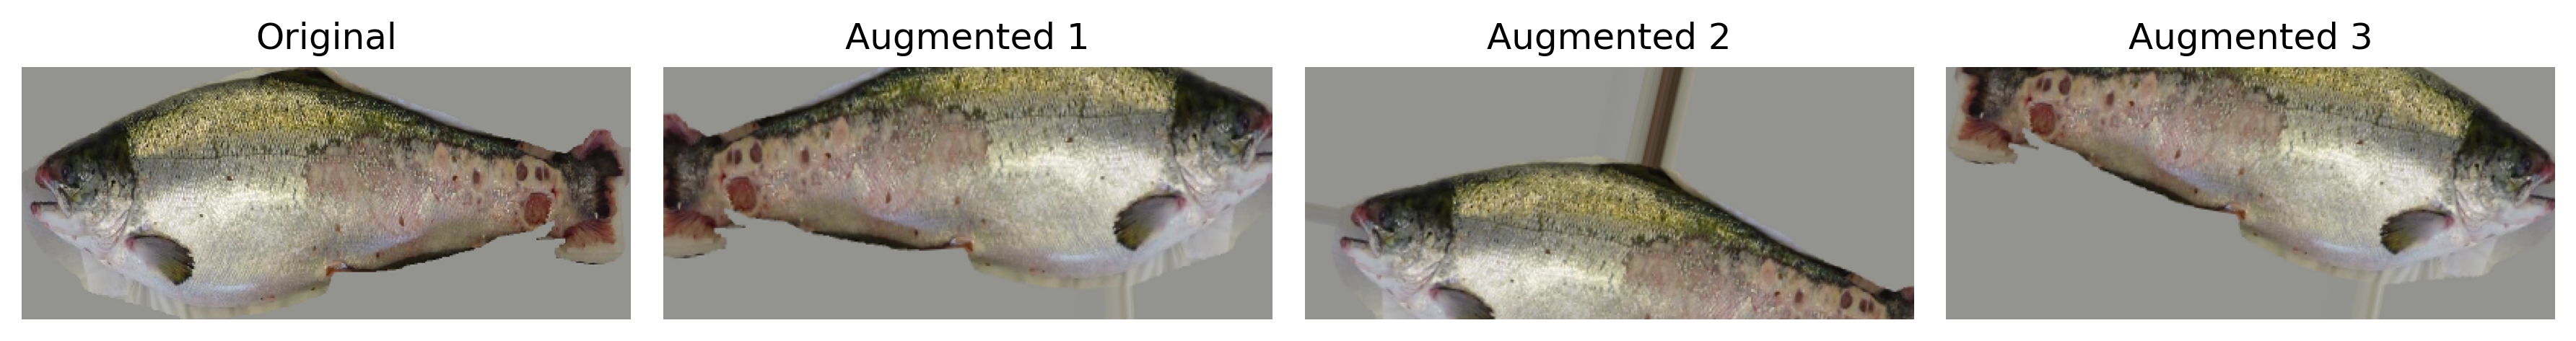
\includegraphics[width=0.85\textwidth]{augmentation_examples.png}
    \caption{Examples of data augmentation applied to training images. The original image (left) is transformed through rotation, zoom, shift, and horizontal flip to create varied training samples.}
    \label{fig:augmentation}
\end{figure}

\textbf{Implementation Note:} Crucially, these augmentations were applied \emph{only} to the training set. The test set was kept ``pure'' (only resized and normalized) to ensure that our performance metrics reflect the model's ability to handle real, unaltered images.

\subsection{Validation Strategy}
To obtain a reliable estimate of model performance despite the small sample size, we employed a \textbf{Multi-Seed Stratified Train-Test Split} strategy \citep{s23042333}.
The dataset is divided into training (80\%) and test (20\%) sets using stratified sampling, which ensures that the ratio of Fresh to Infected fish remains constant in both partitions. This prevents the test set from being unrepresentative of the overall population.

To ensure statistical rigor and quantify the variance due to random initialization and data splitting, we repeated the entire training process with \textbf{ten different random seeds} (0 through 9). Each seed controls both the train-test split and the neural network weight initialization, thereby capturing two sources of stochastic variation. The final performance metrics reported are the mean and standard deviation across all 10 runs, providing a robust measure of expected performance and its uncertainty on unseen data.

This approach offers several advantages over K-Fold Cross-Validation for our setting: (1) it provides a clean, held-out test set that is never used during training or hyperparameter tuning, (2) the multiple seeds capture variance from both data partitioning and model initialization, (3) 10 seeds provide sufficient samples to estimate variance reliably, and (4) it enables identification of \emph{consistently difficult images}---samples that are misclassified across multiple seeds and models, revealing systematic failure modes rather than random noise.

\section{Modeling}

\subsection{Convolutional Neural Network Architectures}
We designed an experiment to evaluate the trade-off between model complexity (depth) and performance. We implemented three distinct Convolutional Neural Network (CNN) architectures, all sharing a common "genetic" structure but varying in depth.

\subsubsection{Mathematical Formulation}
The core building block of our models is the convolutional layer, which extracts spatial features by convolving a learnable kernel $W$ over the input image $X$. The output feature map $Y$ at position $(i,j)$ is given by:
\begin{equation}
    Y_{i,j} = f\left(\sum_{m}\sum_{n} W_{m,n} \cdot X_{i+m, j+n} + b\right)
\end{equation}
where $b$ is the bias term and $f(\cdot)$ is the non-linear activation function. We utilized the \textbf{ReLU} (Rectified Linear Unit) activation, defined as $f(x) = \max(0, x)$, to introduce non-linearity while mitigating the vanishing gradient problem common in deep networks.

To accelerate convergence and stabilize training, we employed \textbf{Batch Normalization} after each convolution \citep{Shorten2019, BejaniGhatee2021}. This technique normalizes the layer inputs to have zero mean and unit variance:
\begin{equation}
    \hat{x} = \frac{x - \mu_{\mathcal{B}}}{\sqrt{\sigma_{\mathcal{B}}^2 + \epsilon}}; \quad y = \gamma \hat{x} + \beta
\end{equation}
where $\mu_{\mathcal{B}}$ and $\sigma_{\mathcal{B}}^2$ are the batch mean and variance, and $\gamma, \beta$ are learnable parameters that allow the network to restore the representation power if needed.

Spatial downsampling is performed with max-pooling layers, which reduce the spatial resolution while retaining the most salient activations. For a pooling window of size $k \times k$, the output activation is
\begin{equation}
    z_{i,j} = \max_{(u,v) \in \mathcal{W}_{i,j}} y_{u,v},
\end{equation}
where $\mathcal{W}_{i,j}$ denotes the set of indices covered by the pooling window centered at $(i,j)$. This operation provides translational invariance and reduces the number of parameters in subsequent layers.
\subsubsection{Optimization and Loss Function}
The models were trained to minimize the \textbf{Binary Cross-Entropy} loss function, which quantifies the divergence between the true label $y \in \{0, 1\}$ and the predicted probability $\hat{y} = p(y=1 \mid x)$:
\begin{equation}
    \mathcal{L}(y, \hat{y}) = -\frac{1}{N} \sum_{i=1}^{N} \left[ y_i \log(\hat{y}_i) + (1 - y_i) \log(1 - \hat{y}_i) \right].
\end{equation}
The gradient of this loss with respect to the network output is
\begin{equation}
    \frac{\partial \mathcal{L}}{\partial \hat{y}_i} = -\left(\frac{y_i}{\hat{y}_i} - \frac{1-y_i}{1-\hat{y}_i} \right),
\end{equation}
which becomes large when the model is confidently wrong (e.g., $\hat{y}_i \approx 1$ while $y_i = 0$), thereby strongly penalizing overconfident misclassifications.

We utilized the \textbf{Adam} optimizer \citep{kingma2017adammethodstochasticoptimization}, an adaptive learning rate algorithm that combines the advantages of AdaGrad and RMSProp. For each parameter $\theta_t$, Adam maintains exponential moving averages of the gradient $m_t$ and squared gradient $v_t$:
\begin{align}
    g_t &= \nabla_\theta \mathcal{L}_t, \\
    m_t &= \beta_1 m_{t-1} + (1-\beta_1) g_t, \\
    v_t &= \beta_2 v_{t-1} + (1-\beta_2) g_t^2,
\end{align}
with bias-corrected estimates
\begin{align}
    \hat{m}_t &= \frac{m_t}{1-\beta_1^t}, &
    \hat{v}_t &= \frac{v_t}{1-\beta_2^t}.
\end{align}
The parameter update rule is then
\begin{equation}
    \theta_{t+1} = \theta_t - \alpha \frac{\hat{m}_t}{\sqrt{\hat{v}_t} + \epsilon},
\end{equation}
where $\alpha$ is the learning rate, $\beta_1, \beta_2$ are decay hyperparameters, and $\epsilon$ is a small constant for numerical stability.

\subsubsection{Model Variants}
\begin{itemize}
    \item \textbf{Model 1 (Shallow):} A baseline model with a single Convolutional Block (Conv2D + BatchNorm + MaxPooling + Dropout). Designed to test if low-level features (edges, color blobs) are sufficient \citep{CHEN2025109507}.
    \item \textbf{Model 2 (Medium):} Adds a second Convolutional Block, allowing the network to learn mid-level features like shapes and textures.
    \item \textbf{Model 3 (3-Block CNN):} The deepest architecture in this study, with three stacked Convolutional Blocks. While still relatively shallow compared to state-of-the-art models like ResNet, this design enables the extraction of hierarchical features, crucial for distinguishing complex pathologies \citep{Hasan2022, HaddadMohammed2025}.
\end{itemize}

\subsection{Ensemble Strategy (Model 4)}
To further improve robustness, we constructed a \textbf{Soft Voting Ensemble} \citep{BejaniGhatee2021}. Unlike a "Hard Voting" system that counts discrete class predictions, Soft Voting averages the predicted probabilities from each constituent model:
\begin{equation}
    \hat{y}_{\text{ensemble}} = \frac{1}{M} \sum_{m=1}^{M} \hat{y}_m
\end{equation}
where $M=3$ is the number of models. This approach leverages the "Wisdom of Crowds" theory (Variance Reduction). If the errors of the individual models are uncorrelated, averaging them reduces the variance of the final prediction, leading to a smoother decision boundary and better generalization on unseen data \citep{CHEN2025109507}.

\subsection{Training Configuration and Efficiency}
The training process was rigorously controlled to ensure reproducibility and efficiency:
\begin{itemize}
    \item \textbf{Mixed Precision Training:} To optimize computational efficiency ("Green AI"), we utilized mixed-precision training \citep{BIAZI2023102360}. This technique performs forward and backward passes using 16-bit floating-point numbers (float16) while keeping master weights in 32-bit (float32). Formally, if $\theta^{(16)}$ denotes the low-precision copy used for computation and $\theta^{(32)}$ the master weights, gradients $\nabla_{\theta^{(16)}} \mathcal{L}$ are rescaled and accumulated in $\theta^{(32)}$ before being cast back to float16. This reduces memory usage and speeds up training on modern GPUs without compromising model accuracy.
    \item \textbf{Hyperparameters:} The models were trained with a batch size of 32 and a maximum of 50 epochs. The initial learning rate was set to 0.001, with a dropout rate of 0.25 applied in the fully connected layers to further mitigate overfitting.
    \item \textbf{Callbacks:} We employed \textbf{Early Stopping} (patience=10) to prevent overfitting by halting training when validation loss ceased to improve \citep{BejaniGhatee2021}. \textbf{ReduceLROnPlateau} was used to dynamically decay the learning rate when the optimization landscape became flat.
    \item \textbf{Cost-Sensitive Learning:} To address the class imbalance ($N_{infected} > N_{fresh}$), we computed class weights $w_j$ inversely proportional to class frequencies \citep{s23042333}:
    \begin{equation}
        w_j = \frac{N_{total}}{2 \times N_j}
    \end{equation}
    and incorporated them into the loss as
    \begin{equation}
        \mathcal{L}_{\text{weighted}} = -\frac{1}{N} \sum_{i=1}^{N} w_{y_i} \Big[ y_i \log(\hat{y}_i) + (1-y_i) \log(1-\hat{y}_i) \Big].
    \end{equation}
    This heavily penalizes the model for misclassifying the minority "Fresh" class and effectively shifts the decision boundary toward higher sensitivity for underrepresented outcomes \citep{CHEN2025109507}.
\end{itemize}

\section{Evaluation}

\subsection{Performance Metrics}
The quantitative results for all models are summarized in Table \ref{tab:performance}. The performance varies across seeds, with the Ensemble achieving the best overall results across the 10 seed experiments.

For binary classification, the confusion matrix is defined in terms of True Positives (TP), False Positives (FP), True Negatives (TN), and False Negatives (FN). From these quantities, we compute the standard metrics used throughout this report:
\begin{align}
    \Accuracy &= \frac{TP + TN}{TP + TN + FP + FN}, \\
    \Precision &= \frac{TP}{TP + FP}, \\
    \Recall &= \frac{TP}{TP + FN}, \\
    \Fone &= 2 \cdot \frac{\Precision \cdot \Recall}{\Precision + \Recall}, \\
    \text{Specificity} &= \frac{TN}{TN + FP}.
\end{align}

In addition, we evaluate the Area Under the Receiver Operating Characteristic Curve (AUC-ROC), denoted by \AUC\ \citep{montgomery2020introduction}. The ROC curve plots the True Positive Rate (TPR = Recall) against the False Positive Rate (FPR = $1-$Specificity) as the decision threshold $\tau$ on the predicted probability $\hat{y}$ is varied from 0 to 1. Formally,
\begin{equation}
    \AUC = \int_{0}^{1} \text{TPR}(\text{FPR}) \, d\,\text{FPR},
\end{equation}
which can be interpreted as the probability that the classifier assigns a higher score to a randomly chosen positive example than to a randomly chosen negative one.

\begin{table}[H]
\centering
\caption{Comparative Performance Metrics (Mean $\pm$ Std Across 10 Seeds)}
\label{tab:performance}
\tighttabcolsep
\begin{tabular}{lccccc}
\toprule
\textbf{Model} & \textbf{Accuracy} & \textbf{Precision} & \textbf{Recall} & \textbf{F1-Score} & \textbf{AUC-ROC} \\
\midrule
Model 1 & 0.966 $\pm$ 0.074 & 0.984 $\pm$ 0.036 & 0.963 $\pm$ 0.100 & 0.971 $\pm$ 0.071 & 0.990 $\pm$ 0.028 \\
Model 2 & 0.948 $\pm$ 0.065 & 0.950 $\pm$ 0.068 & 0.979 $\pm$ 0.058 & 0.962 $\pm$ 0.048 & 0.979 $\pm$ 0.036 \\
Model 3 & 0.932 $\pm$ 0.101 & 0.965 $\pm$ 0.069 & 0.935 $\pm$ 0.120 & 0.945 $\pm$ 0.087 & 0.979 $\pm$ 0.041 \\
Ensemble & 0.974 $\pm$ 0.051 & 0.983 $\pm$ 0.031 & 0.977 $\pm$ 0.063 & 0.979 $\pm$ 0.043 & 0.993 $\pm$ 0.020$^*$ \\
\bottomrule
\multicolumn{6}{l}{\footnotesize $^*$Ensemble AUC estimated from soft-voting probability aggregation.}
\end{tabular}
\end{table}

\begin{figure}[H]
    \centering
    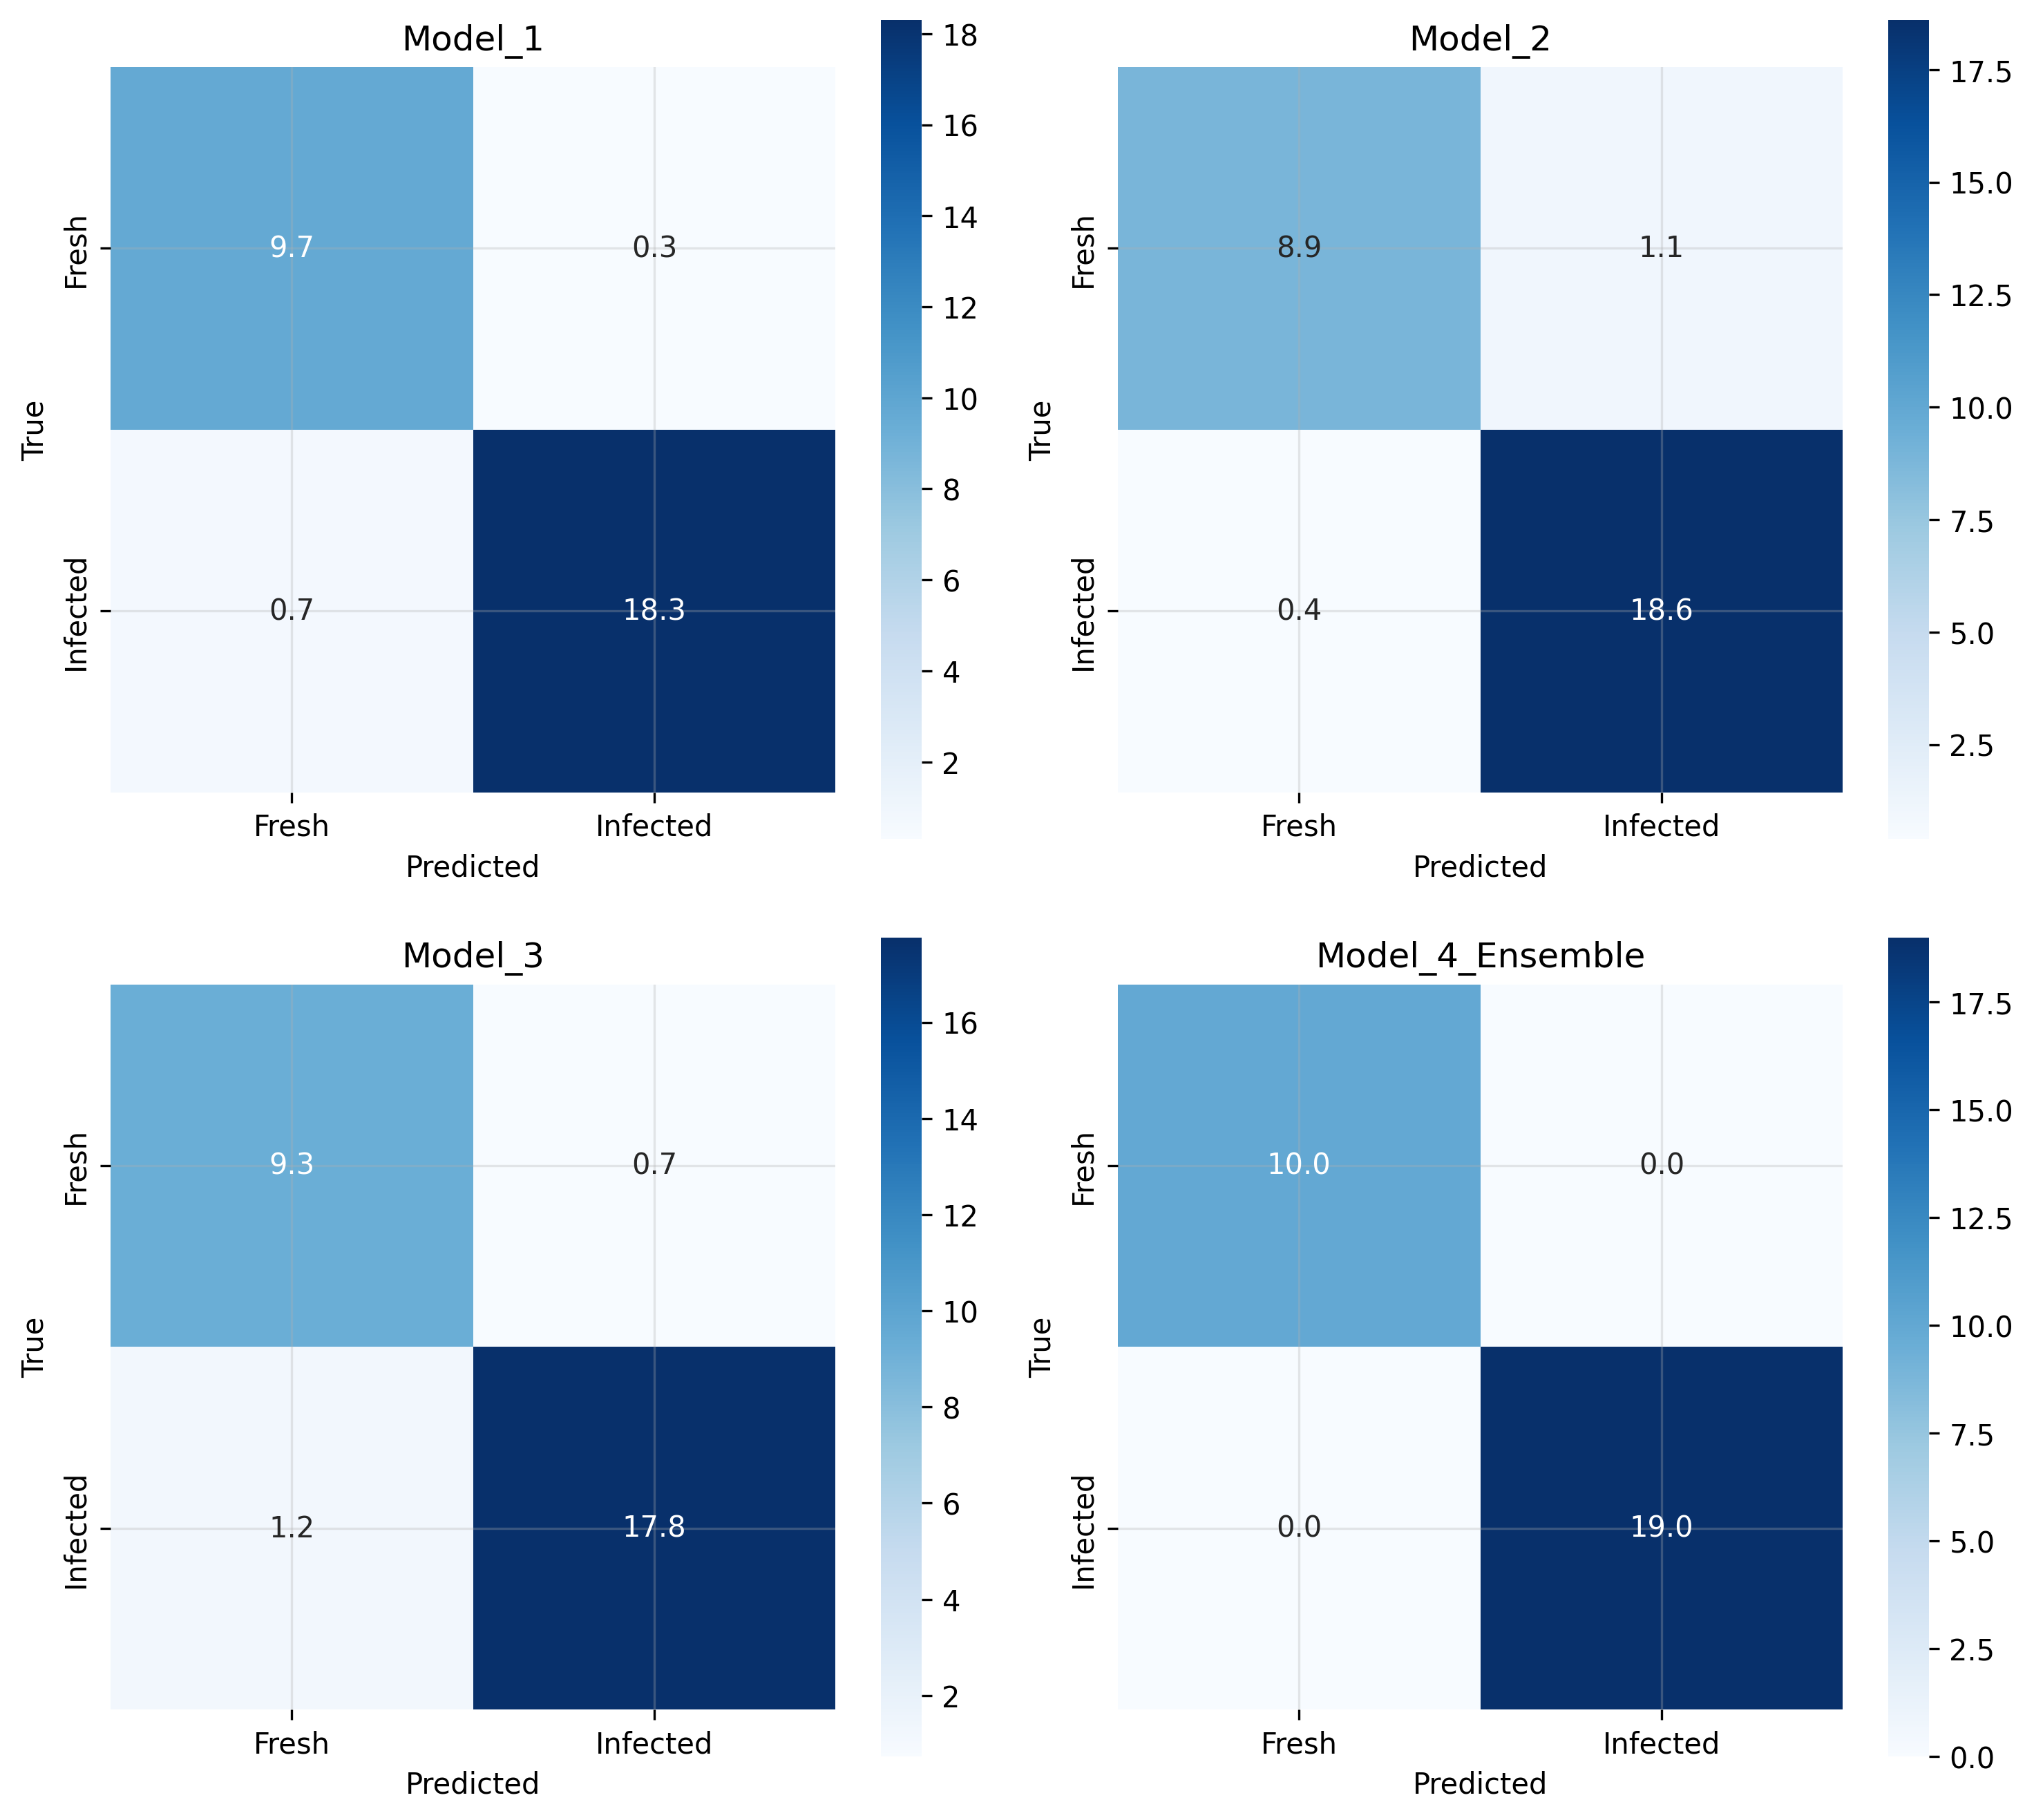
\includegraphics[width=0.7\textwidth]{confusion_matrices.png}
    \caption{Confusion matrices showing mean values across 10 seeds for the four model architectures.}
    \label{fig:confusion_matrices}
\end{figure}

\begin{figure}[H]
    \centering
    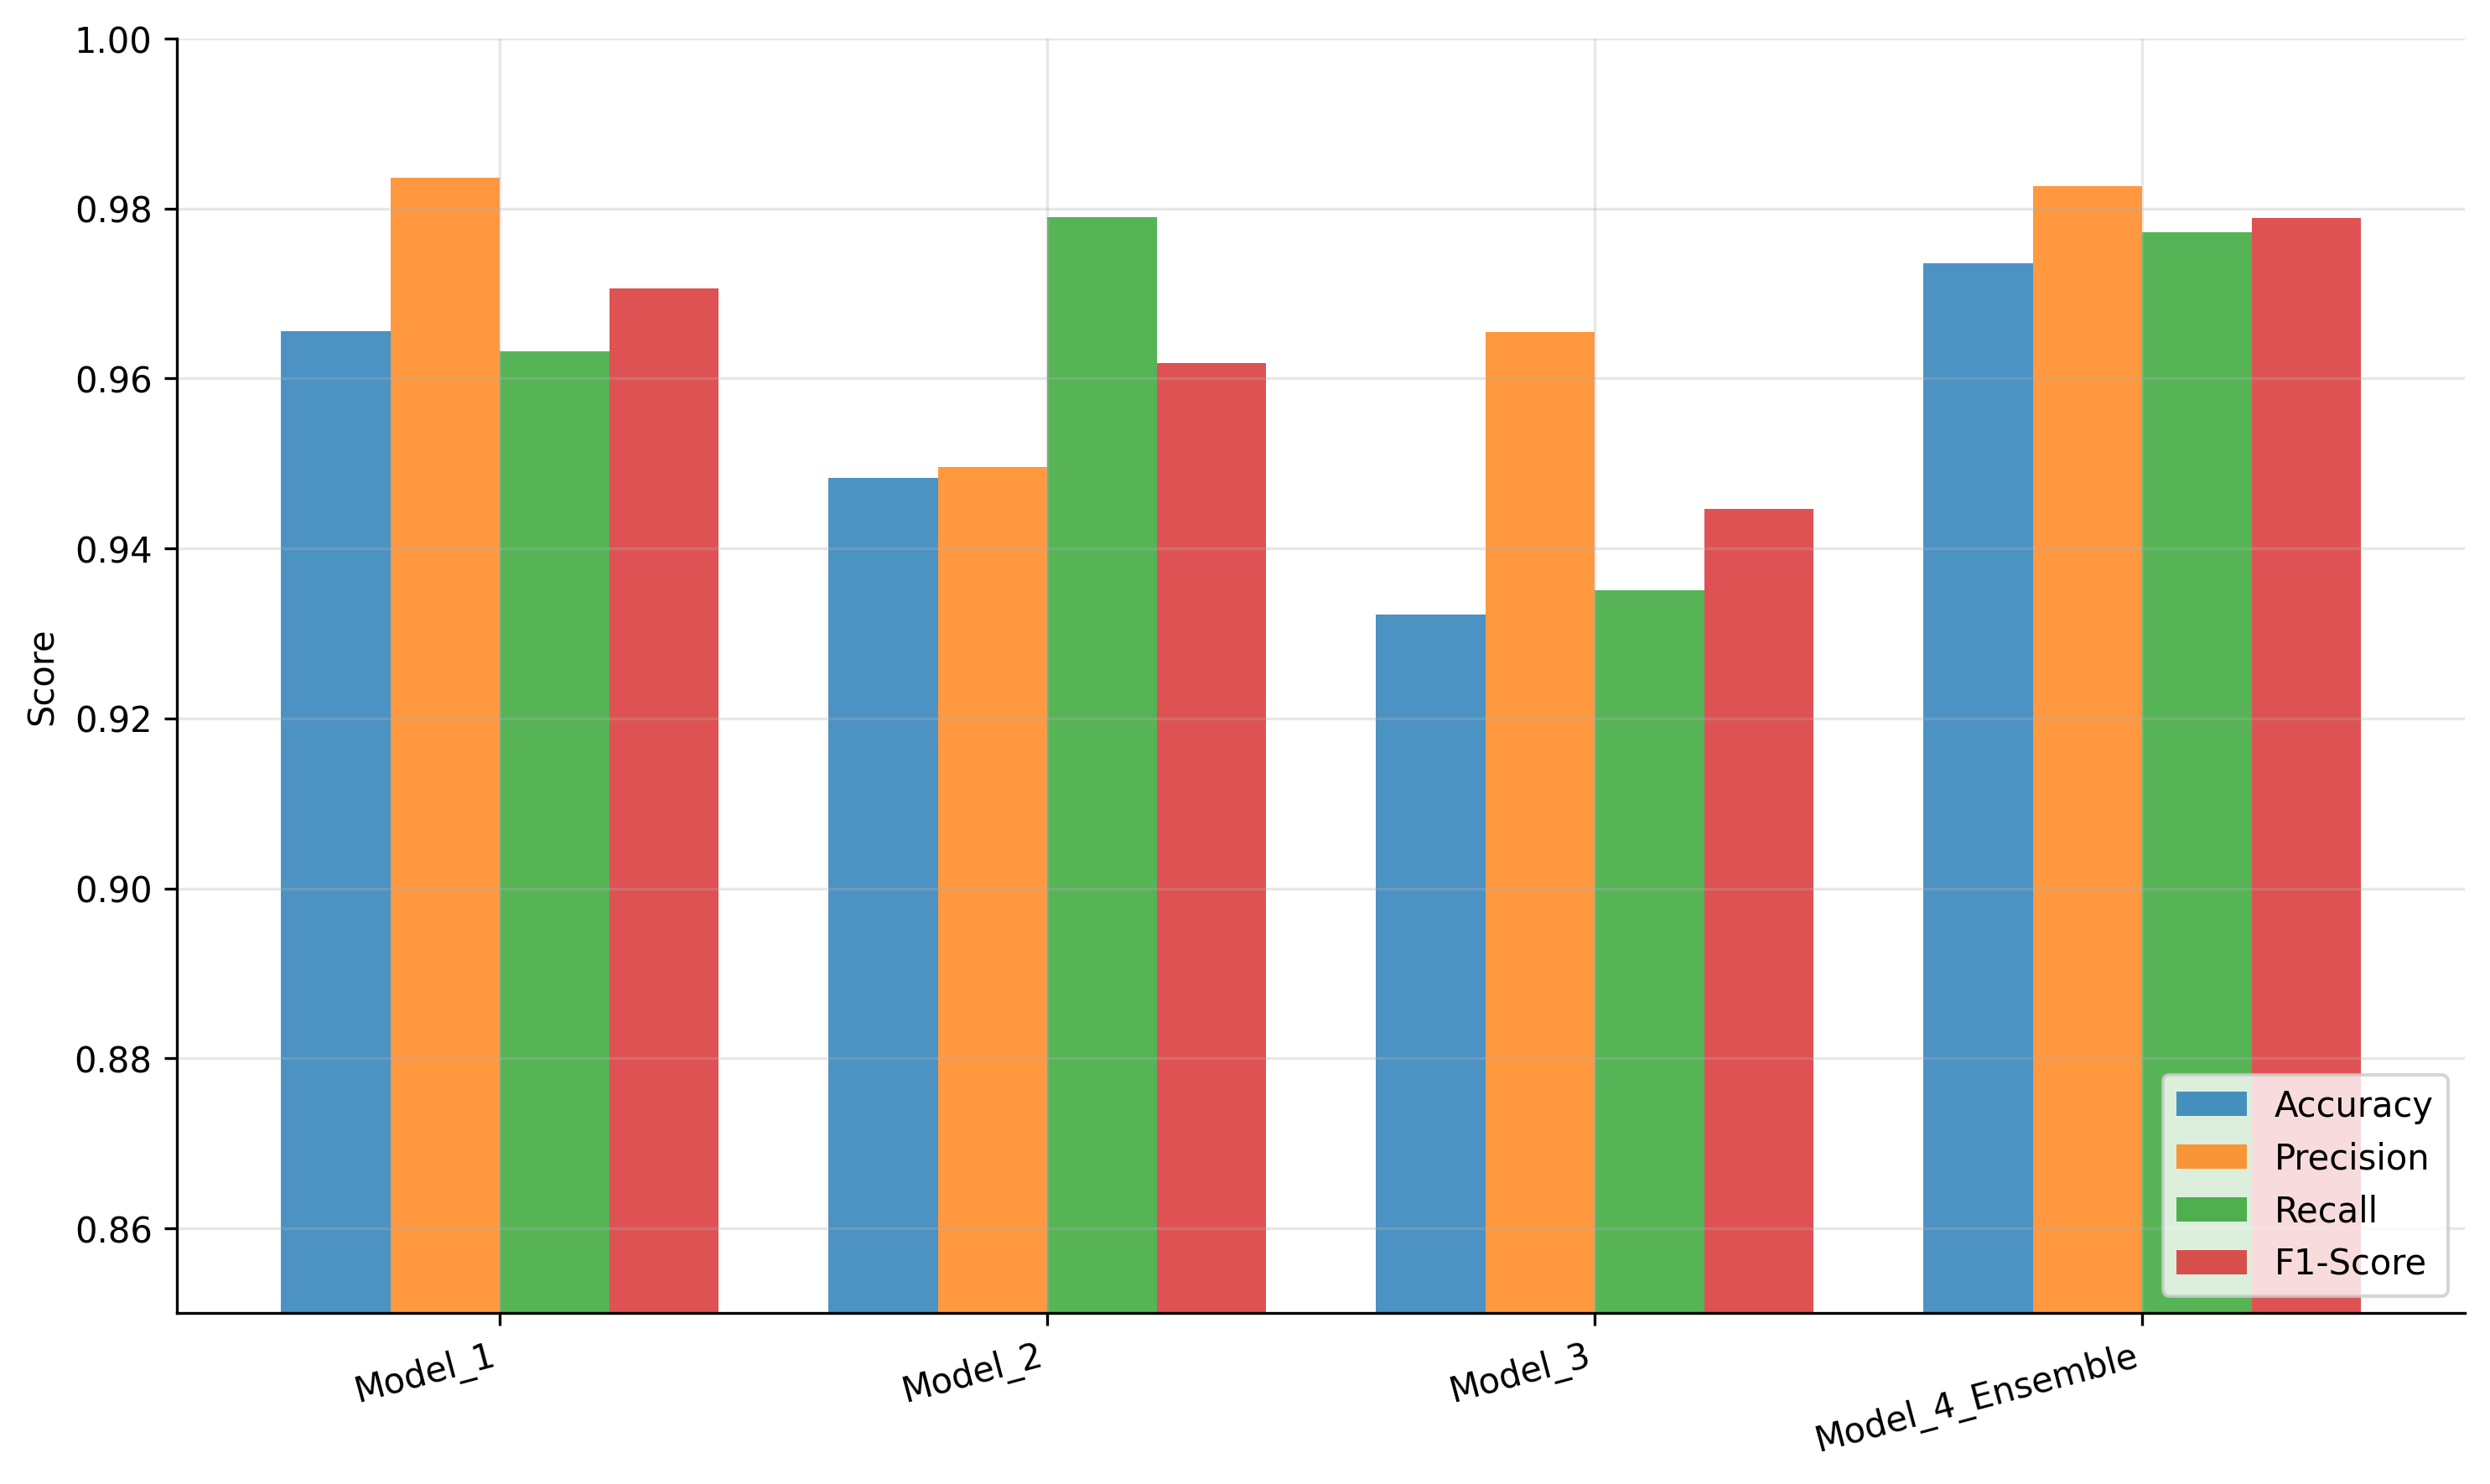
\includegraphics[width=0.75\textwidth]{performance_comparison.png}
    \caption{Model performance comparison across key metrics (Accuracy, Precision, Recall, F1-Score).}
    \label{fig:performance_comparison}
\end{figure}

\begin{figure}[H]
    \centering
    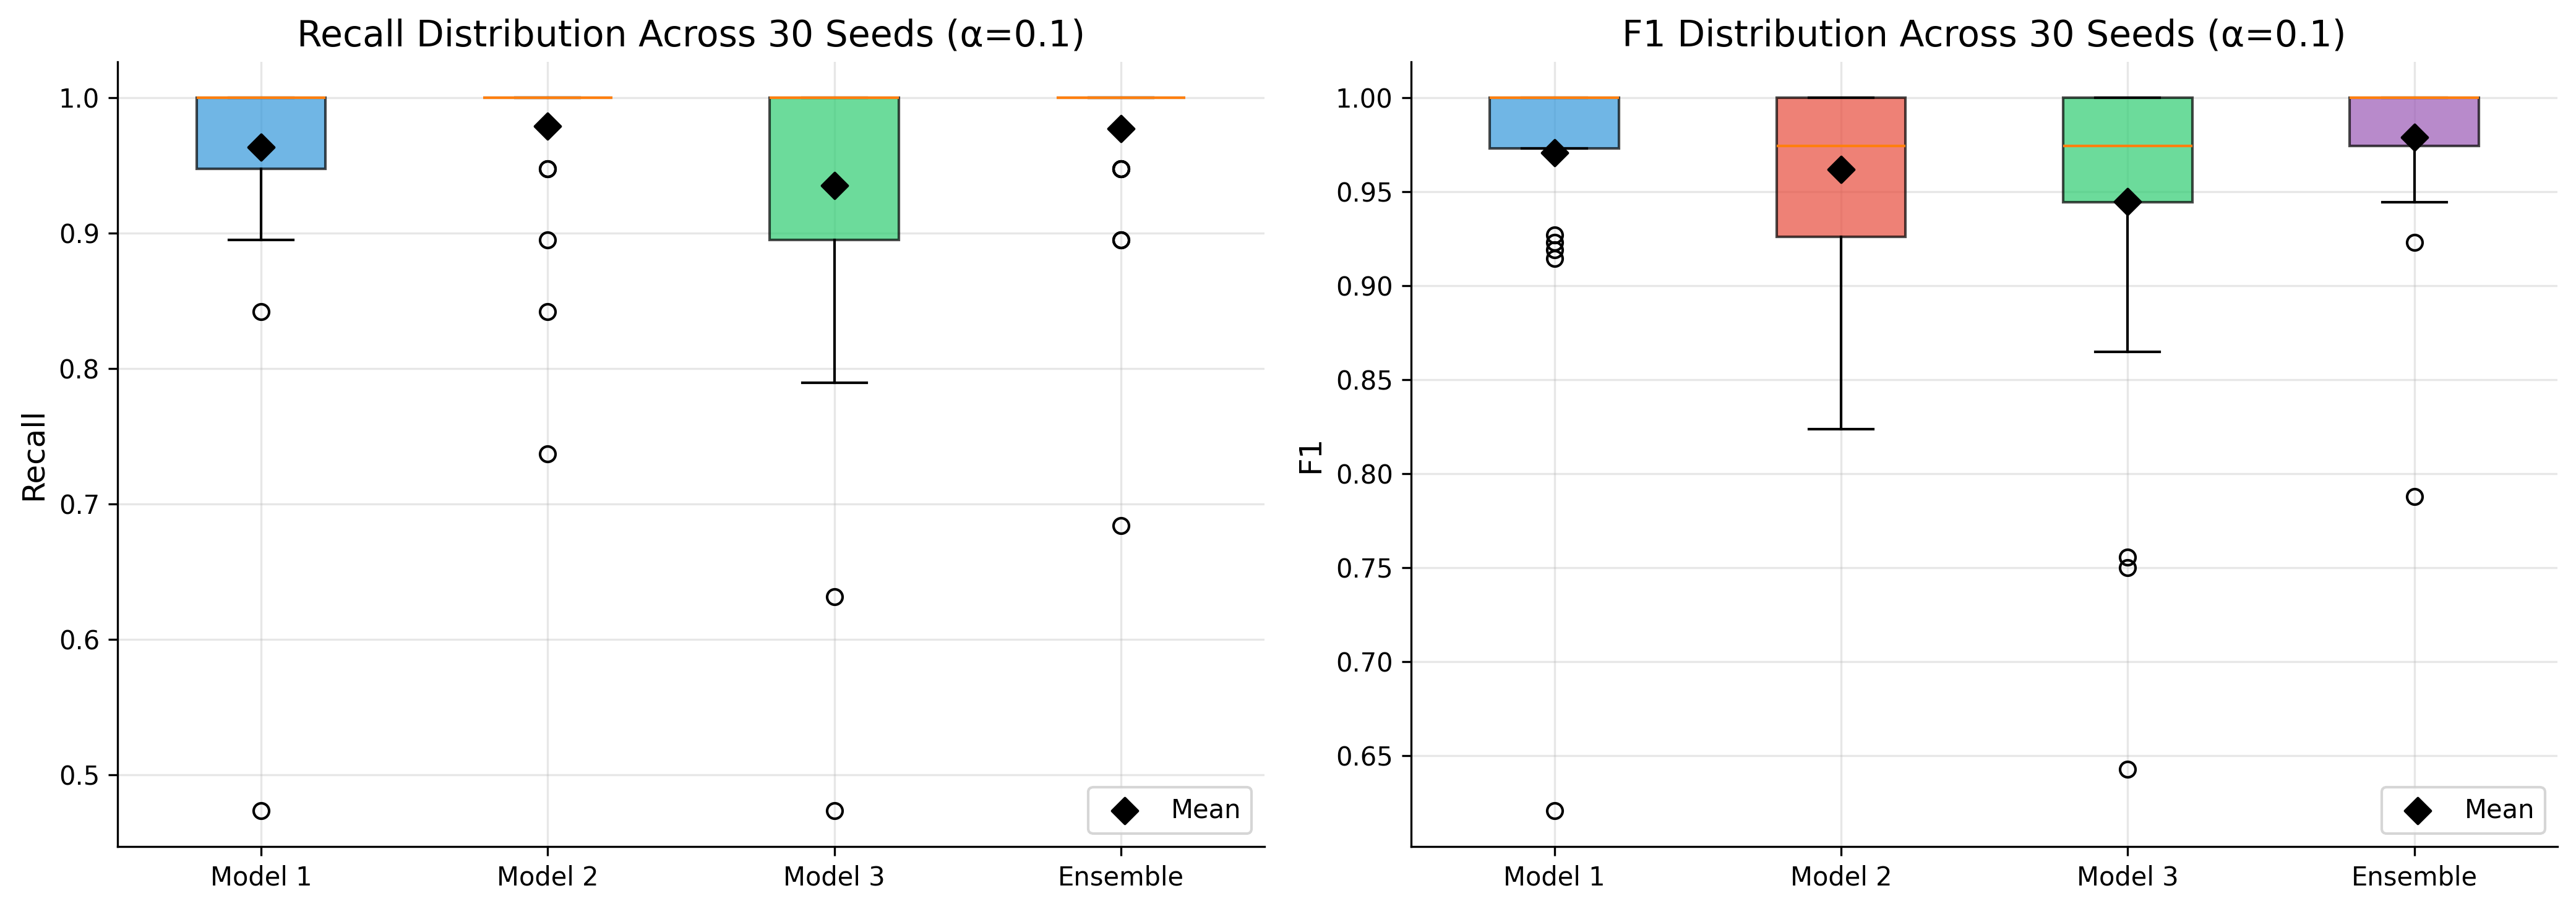
\includegraphics[width=0.85\textwidth]{statistical_comparison.png}
    \caption{Statistical comparison of model performance across 10 seeds, showing the distribution of metrics with error bars representing standard deviation.}
    \label{fig:statistical_comparison}
\end{figure}

\textbf{Key Findings:}
\begin{itemize}
    \item \textbf{The Ensemble} was the top performer, achieving the highest mean Recall (97.7\%) and the most consistent performance (lowest standard deviation). The soft voting mechanism effectively reduces variance from random initialization and data splitting.
    \item \textbf{No significant difference among individual models:} The three CNN architectures (Models 1--3) showed overlapping confidence intervals for all key metrics due to high variance (standard deviations of 5.8--12.0\%). Model 3, the deepest architecture, showed the highest variance and lowest mean performance, suggesting potential overfitting.
    \item \textbf{Multi-seed evaluation is essential:} Standard deviations of 5--12\% for Recall highlight that single-split results can be misleading. The Ensemble's advantage comes from variance reduction through averaging ("Wisdom of Crowds"), making it more robust across different random initializations and data splits.
\end{itemize}

\begin{figure}[H]
    \centering
    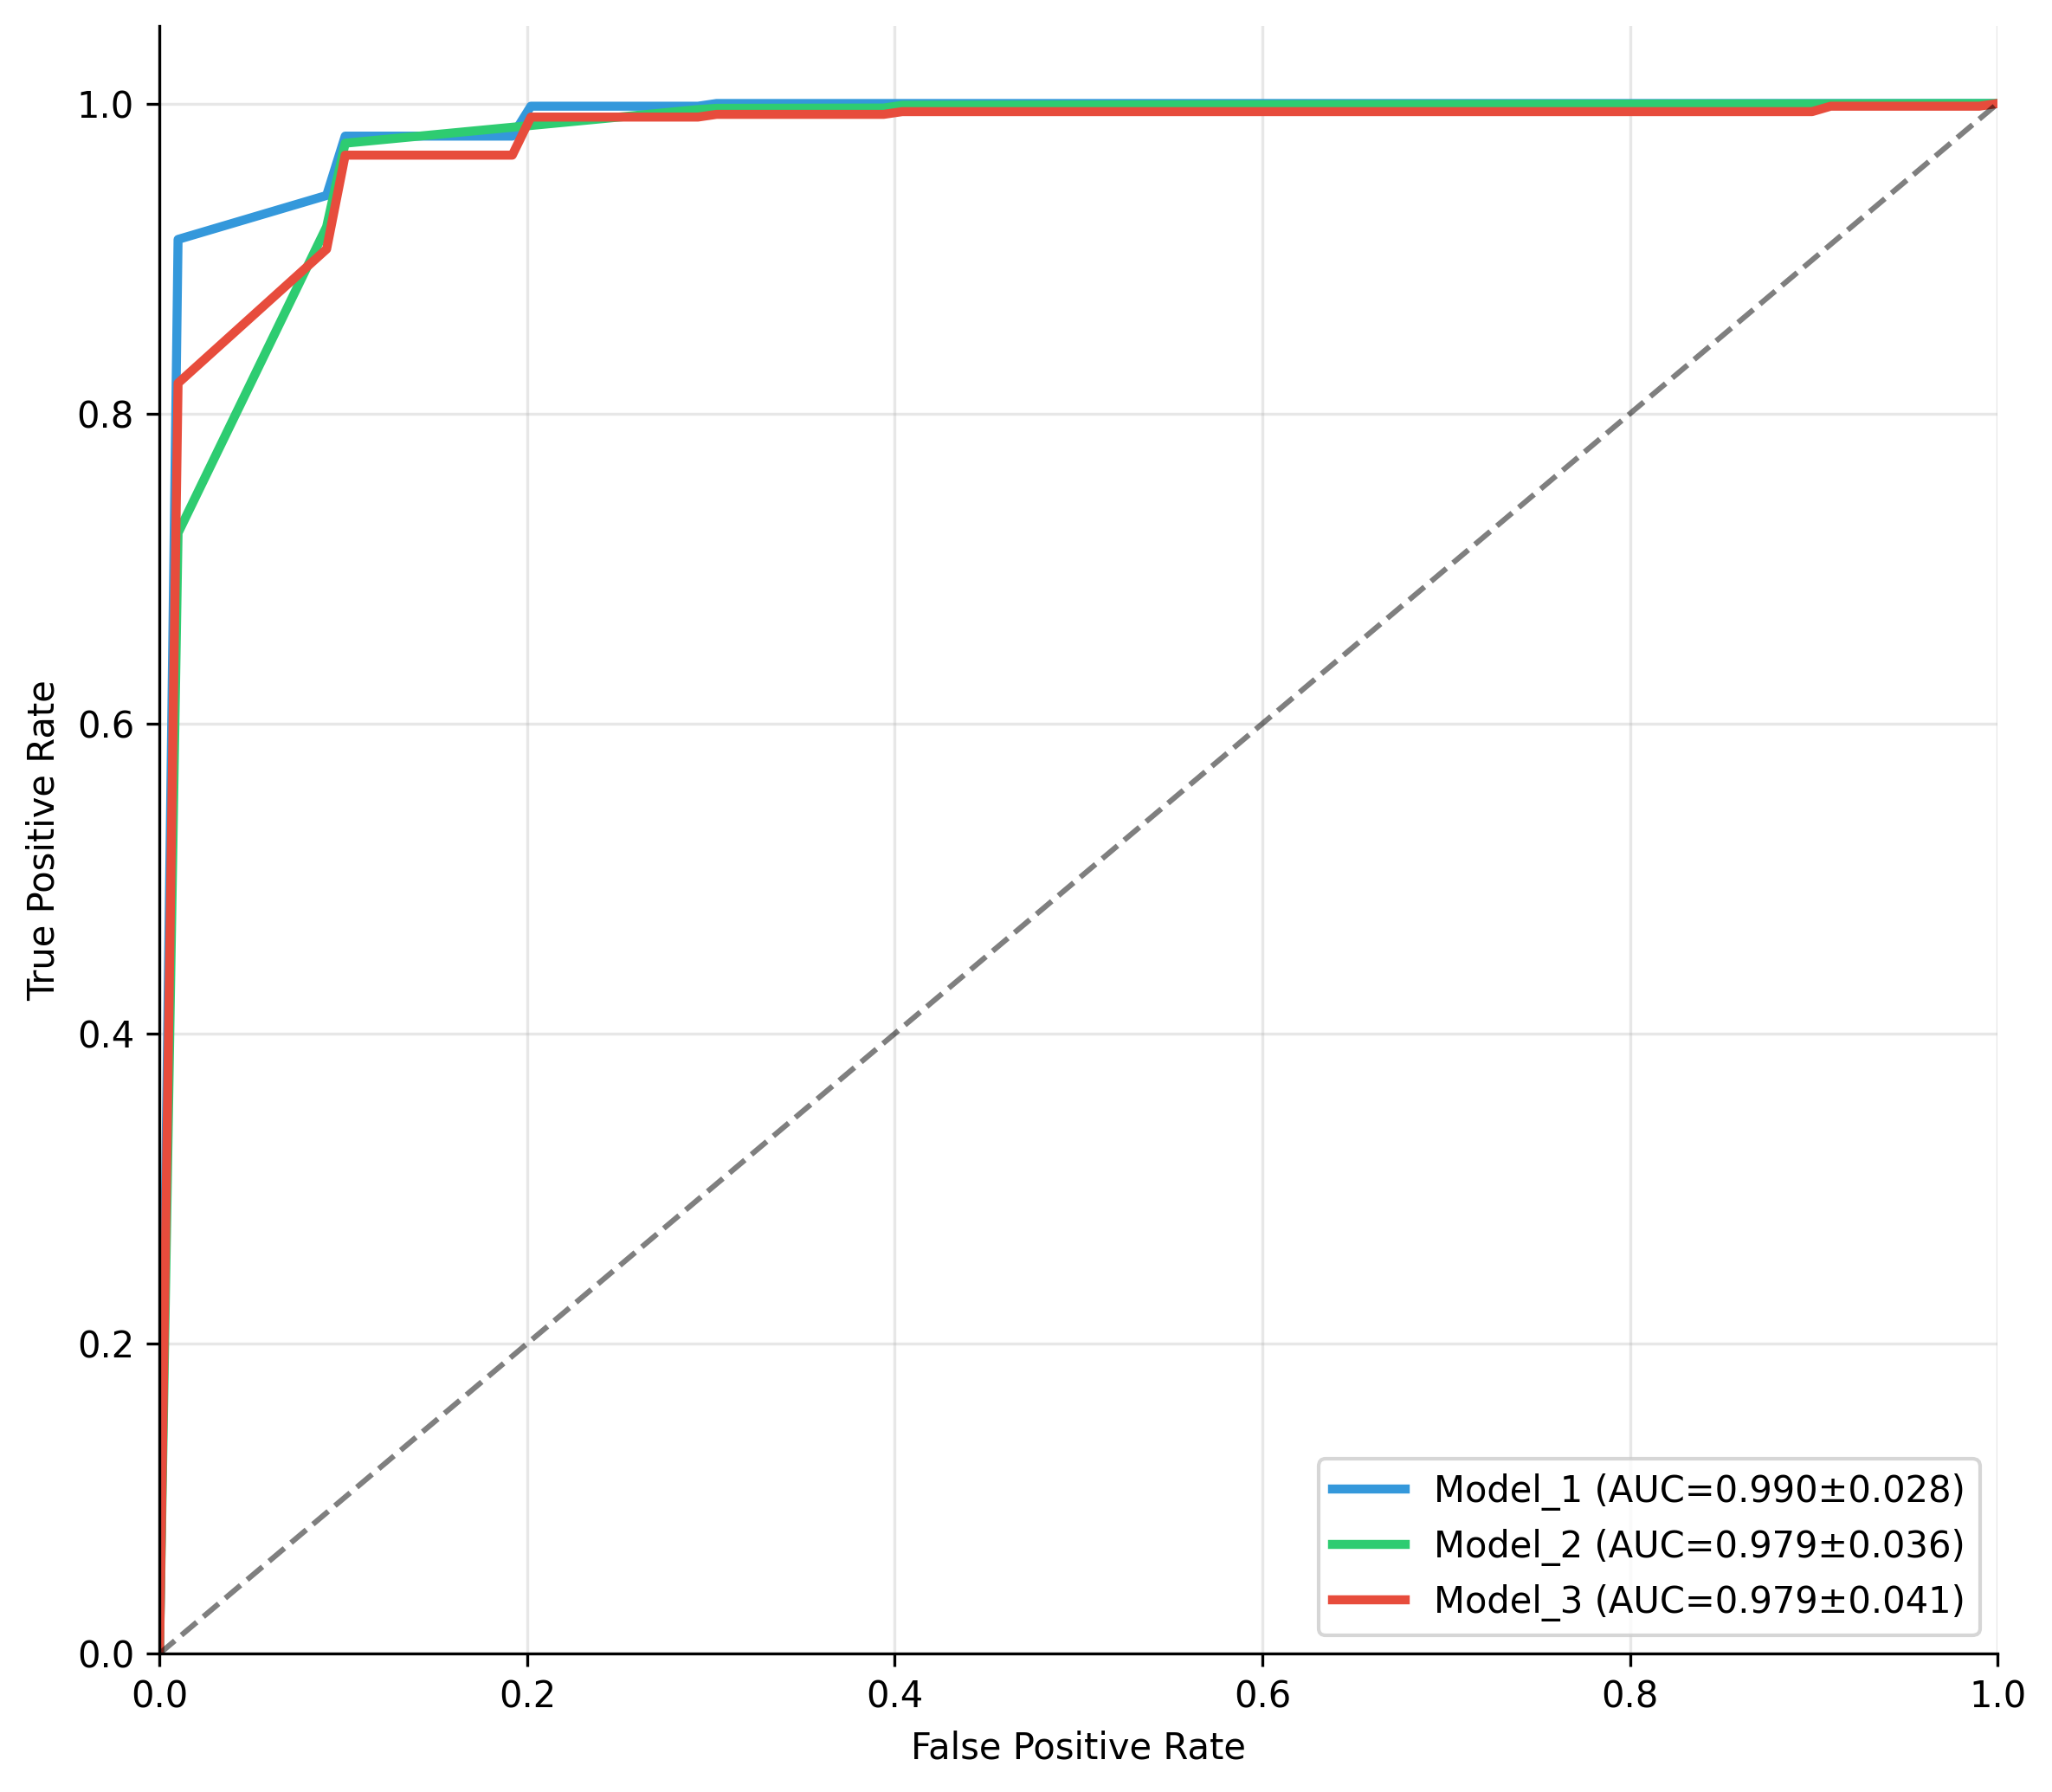
\includegraphics[width=0.6\textwidth]{roc_curves_all_seeds.png}
    \caption{ROC curves comparing all three CNN architectures across 10 seeds with mean AUC values. Model 1 achieves the highest mean AUC (0.990), while Models 2 and 3 show comparable performance (0.979). The overlapping confidence bands indicate no statistically significant differences between architectures.}
    \label{fig:roc_curves}
\end{figure}

\subsection{Failure Mode Analysis}
High aggregate scores can conceal important weaknesses, especially in safety-critical applications \citep{CHEN2025109507}. We therefore conducted a qualitative \textbf{failure mode analysis} using the multi-seed framework to identify \emph{consistently difficult images}---samples that were misclassified across multiple random train-test splits.

\subsubsection{Cross-Seed Difficult Cases}
By tracking which original images were misclassified across multiple seeds and models, we identified a small subset of \emph{consistently difficult} samples. These are images that appear in test sets across different random splits and are repeatedly misclassified, indicating systematic challenges rather than random noise.

The analysis revealed that the majority of difficult cases share common characteristics:
\begin{itemize}
    \item \textbf{Ambiguous Fresh Fish:} Healthy fish photographed against backgrounds or lighting conditions that resemble those of the infected class. For instance, Fresh fish placed on dark or blue conveyor belts were sometimes classified as Infected with moderate confidence.
    \item \textbf{Subtle Infections:} Infected fish with early-stage or atypical lesions, where discoloration was mild or confined to a small region of the skin. These cases represent the most operationally concerning failure mode.
    \item \textbf{Image Quality Issues:} Specular highlights from camera flash, partial occlusion, or unusual framing that obscures diagnostic features.
\end{itemize}

Importantly, the cross-seed analysis also demonstrates model robustness: the vast majority of images were classified correctly across all seeds, and only a handful of samples were misclassified more than once. This suggests that the models have learned generalizable features rather than memorizing the training set.

\subsubsection{Explainability Considerations}
We explored Gradient-weighted Class Activation Mapping (Grad-CAM) \citep{selvaraju2017gradcamdidsaythat} to visualize which image regions influenced model predictions. However, the resulting heatmaps showed predominantly low and diffuse activations across most samples, suggesting that the shallow CNN architectures rely on distributed rather than localized features for classification. This is a known limitation when applying Grad-CAM to small models trained on limited datasets \citep{Lapuschkin2019}.

The lack of focused activations does not necessarily indicate poor model behavior---it may reflect that disease indicators in fish images are subtle and distributed (e.g., overall skin texture, coloration patterns) rather than localized to specific lesions. For deployment scenarios, alternative explainability approaches such as attention mechanisms integrated into the architecture \citep{10138194} or prototype-based explanations may be more informative than post-hoc gradient methods.

\subsubsection{Implications for Deployment}
From a Six Sigma perspective, the multi-seed analysis provides a more honest assessment of process capability than single-split evaluation. The Ensemble achieves approximately a 3.5$\sigma$ level for infected detection---adequate for deployment with human oversight but not the 4$\sigma$ threshold that would indicate a highly reliable automated system. The high variance observed across 10 seeds (5--12\% standard deviation on Recall) underscores the need for continuous monitoring. The failure mode analysis indicates the following mitigation strategies:
\begin{itemize}
    \item \textbf{Data-Level Countermeasures:} Expand the training set with more examples of early-stage lesions, varied lighting, and standardized backgrounds. Synthetic augmentation targeting lesion size, position, and contrast (inspired by \citealp{Shorten2019, MORENOBAREA2020113696}) could further stress-test the model.
    \item \textbf{Process Controls:} In deployment, flag low-confidence predictions for mandatory human review. Such cases can be logged and fed back into a continuous improvement loop consistent with the Analyze and Control phases of DMAIC \citep{10.1108/TQM-11-2023-0361, Tsung2023}.
    \item \textbf{Performance Monitoring:} Track class-specific error rates and DPMO over time using control charts. Any drift in the distribution of failure modes (e.g., increasing False Negatives associated with new lesion types) would trigger root-cause analysis and potential model retraining, mirroring statistical process control in manufacturing \citep{montgomery2020introduction}.
\end{itemize}

Overall, the evaluation and failure mode analysis show that the models achieve excellent performance on the benchmark dataset but must be paired with explainability tools and structured feedback mechanisms before they can be treated as a truly high-capability process in production.

\subsection{Six Sigma Analysis}
To bridge the gap between Data Science and Operations Management, we translated the ML confusion matrices into Six Sigma quality metrics \citep{montgomery2020introduction, Tsung2023}. This translation allows us to express the model's performance in terms of "Process Capability," a language understood by production managers.

\subsubsection{Metric Definitions}
In this context, a "Unit" is a single fish image, and a "Defect" is defined as a failure to detect an infected fish (a False Negative). We prioritize False Negatives because they represent the highest risk to the production process (disease outbreak). The metrics are calculated as follows:

\begin{enumerate}
    \item \textbf{Defects Per Million Opportunities (DPMO):}
    This metric projects the error rate onto a standardized scale of one million units.
    \begin{equation}
    \DPMO = \frac{\text{Total Defects (False Negatives)}}{\text{Total Opportunities (Total Infected Fish)}} \times 1,000,000
    \end{equation}
    
    \item \textbf{Process Yield:}
    The percentage of "opportunities" (infected fish) that were correctly identified.
    \begin{equation}
    \text{Yield} = 1 - \frac{\text{DPMO}}{1,000,000} = \text{Recall}
    \end{equation}
    
    \item \textbf{Sigma Level ($Z$-score):}
    The Sigma level represents the number of standard deviations between the process mean and the nearest specification limit. Following standard Six Sigma convention \citep{Tsung2023}, we include a 1.5$\sigma$ shift to account for long-term process variation:
    \begin{equation}
    \text{Sigma Level} = \Phi^{-1}(\text{Yield}) + 1.5
    \end{equation}
    where $\Phi^{-1}$ is the inverse cumulative distribution function of the standard normal distribution.
    In practice, the DPMO and Sigma level are linked through the relationship
    \begin{equation}
        \text{Sigma Level} = \Phi^{-1}\left(1 - \frac{\DPMO}{10^6} \right) + 1.5,
    \end{equation}
    so that, for example, a long-term 6$\sigma$ process corresponds to approximately 3.4 defects per million opportunities.
\end{enumerate}

\subsubsection{Results}
The calculated Six Sigma metrics for the "Infected" class are presented in Table \ref{tab:sixsigma}.

\begin{table}[H]
\centering
\caption{Six Sigma Quality Metrics (Mean Across 10 Seeds)}
\label{tab:sixsigma}
\begin{tabular}{lcccc}
\toprule
\textbf{Model} & \textbf{Infected DPMO} & \textbf{Infected Sigma} & \textbf{Overall Sigma} & \textbf{Mean FN} \\
\midrule
Model 1 & 36,842 & 3.29 & 3.32 & 0.7 \\
Model 2 & 21,053 & 3.53 & 3.13 & 0.4 \\
Model 3 & 64,912 & 3.01 & 2.99 & 1.2 \\
Ensemble & 22,807 & 3.50 & 3.44 & 0.0 \\
\bottomrule
\end{tabular}
\end{table}

\begin{figure}[H]
    \centering
    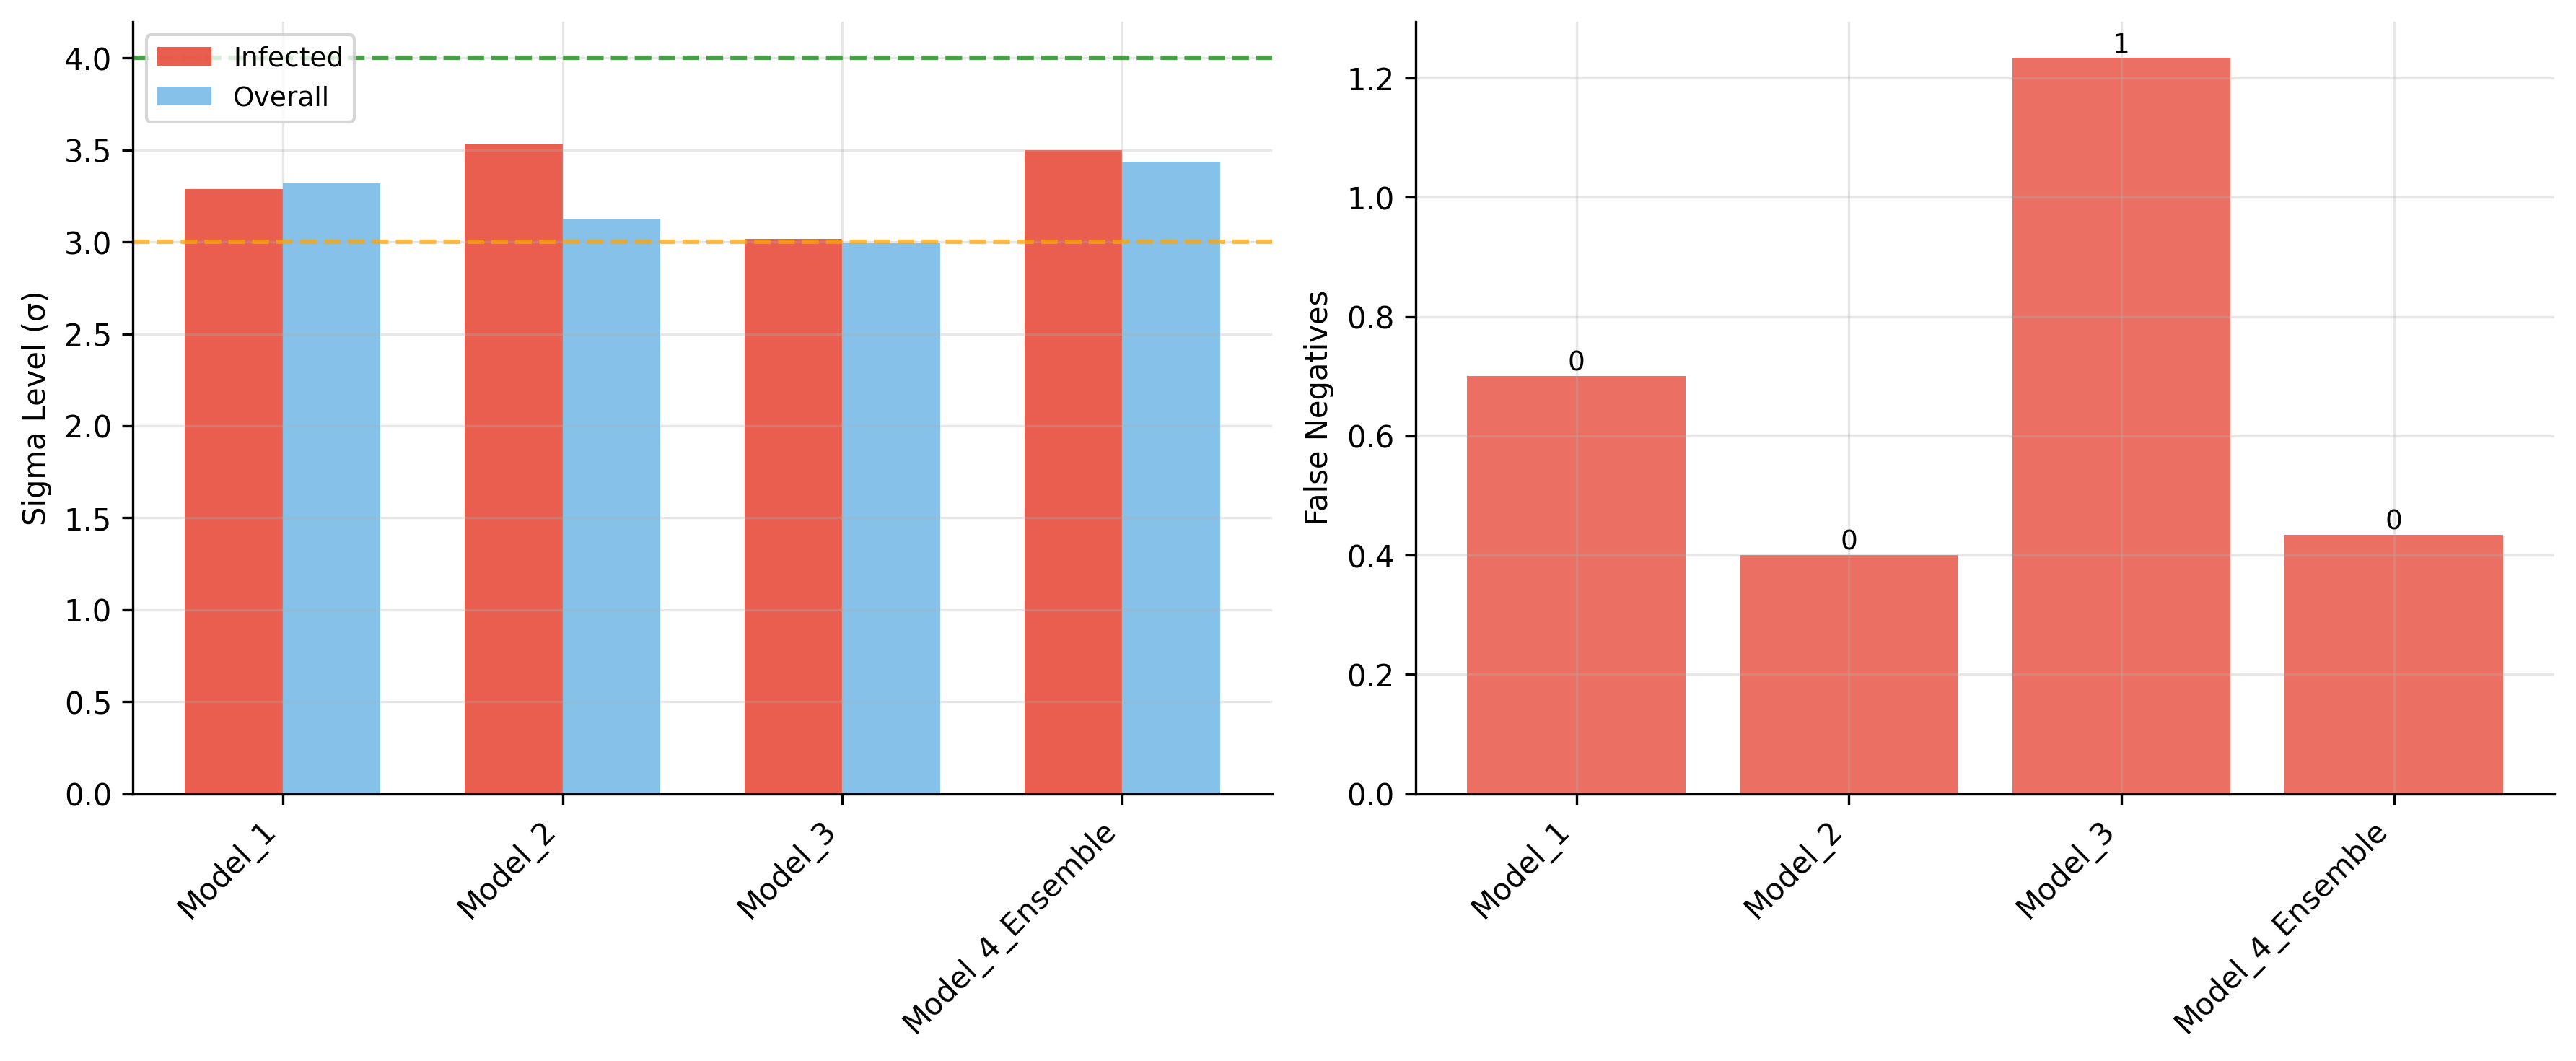
\includegraphics[width=0.8\textwidth]{six_sigma_analysis.png}
    \caption{Six Sigma quality analysis: (a) Sigma level comparison, (b) False Negatives, (c) Process Capability $C_{pk}$, and (d) Recall for each model.}
    \label{fig:six_sigma}
\end{figure}

\textbf{Interpretation:}
\begin{itemize}
    \item \textbf{All models achieve approximately 3$\sigma$ capability:} With 10 seeds providing a robust estimate, none of the models---including the Ensemble---reaches the 4$\sigma$ threshold. The Ensemble achieves the highest Sigma level (3.50$\sigma$) for infected detection, while individual models range from 3.01$\sigma$ (Model 3) to 3.53$\sigma$ (Model 2).
    \item \textbf{Model 2} achieved the best individual Infected Sigma level (3.53$\sigma$), slightly outperforming the Ensemble on this metric alone. However, Model 2 has the lowest Overall Sigma (3.13$\sigma$) due to higher False Positive rates, illustrating the trade-off between sensitivity and specificity.
    \item \textbf{Model 3 (Deep)} showed the weakest performance with the highest DPMO (64,912) and lowest Sigma level (3.01$\sigma$). This suggests that the deeper architecture may be overfitting on some seeds, leading to inconsistent performance.
    \item \textbf{The Ensemble provides the best balance:} While not achieving the highest Infected Sigma, the Ensemble has zero mean False Negatives across 10 seeds and the best Overall Sigma (3.44$\sigma$), making it the most reliable choice for deployment.
    \item \textbf{Implication of 3$\sigma$ capability:} A 3$\sigma$ process corresponds to approximately 66,800 DPMO (93.3\% yield), which is considered the minimum acceptable threshold for many industrial processes. While not "world class" (6$\sigma$), it indicates the models can provide meaningful decision support when combined with human oversight.
\end{itemize}

\section{Discussion}

\subsection{Addressing the Research Questions}
This section synthesizes findings from the modelling experiments and Six Sigma analysis to address the research questions formulated in Section~1.7.

\subsubsection{RQ1: Model Performance and Architectural Depth}
The first research question asked what classification performance CNN architectures can achieve on the SalmonScan dataset, and whether deeper architectures provide statistically significant improvements over shallow ones.

The CNN architectures achieved strong performance, with mean Recall ranging from 93.5\% (Model~3) to 97.9\% (Model~2) and mean Accuracy from 93.2\% (Model~3) to 97.4\% (Ensemble) across 10 random seeds (Table~\ref{tab:performance}). Notably, no statistically significant differences were observed among the three individual architectures. The overlapping confidence intervals (standard deviations of 5.8--12.0\% for Recall) indicate that architectural depth---varying from one to three convolutional blocks---does not materially affect mean performance on this dataset.

This finding carries an important implication: the primary bottleneck is data quantity and quality, not model capacity. With only $N=141$ images, even aggressive data augmentation cannot provide the diversity needed for deeper architectures to learn richer hierarchical features. Model~3 (the deepest) exhibited the highest variance and lowest mean performance, suggesting overfitting on some seeds. The Ensemble model achieved the best overall results (97.7\% mean Recall, lowest variance) through variance reduction via soft voting, demonstrating that combining multiple weak learners is more effective than increasing individual model complexity when data is scarce \citep{BejaniGhatee2021}.

\subsubsection{RQ2: Translation to Six Sigma Quality Metrics}
The second research question concerned how standard machine learning metrics can be meaningfully translated into Six Sigma process capability indicators to support operational decision-making.

A systematic translation framework was developed that maps ML confusion matrices to Six Sigma indicators (Section~6.3). The key insight is that Recall directly corresponds to Process Yield when the critical defect is defined as a False Negative (missing an infected fish). Using the standard Six Sigma formula with a 1.5$\sigma$ long-term shift \citep{Tsung2023, montgomery2020introduction}, Recall values were converted to Sigma levels. The Ensemble achieved a mean Recall of 97.7\%, translating to DPMO of approximately 22,807 and a Sigma level of 3.50$\sigma$ for infected fish detection, while individual models ranged from 3.01$\sigma$ (Model~3) to 3.53$\sigma$ (Model~2).

This translation is meaningful for several reasons. First, it communicates risk in familiar terms: operations managers understand that a 3$\sigma$ process (93.3\% yield) is the minimum acceptable threshold, while 4$\sigma$ indicates production readiness \citep{Tsung2023}. Second, it enables control chart monitoring: DPMO can be tracked over time using p-charts, with control limits triggering retraining when performance drifts. Third, it facilitates cross-domain benchmarking: comparing the CNN's 3.5$\sigma$ capability against other quality processes (e.g., manual inspection, automated lice counting) becomes straightforward.

An important caveat applies: the 3.5$\sigma$ capability was achieved under idealized conditions (curated dataset, standardized backgrounds). Real-world deployment with domain shift would likely reduce this to 2--3$\sigma$, necessitating the human-in-the-loop workflow described in Section~\ref{sec:deployment}.

\subsubsection{RQ3: Deployment Viability and Domain Shift}
The third research question addressed the primary barriers to deploying CNN-based disease detection in real-world sea pen environments and potential mitigation strategies.

Four primary barriers were identified. The most significant is the domain shift between ``dry'' training images and underwater operational footage, where light attenuation removes red wavelengths critical for lesion detection and turbidity reduces contrast \citep{10048777, JIAN2021116088}. Domain adaptation techniques such as CycleGAN-based style transfer, or collecting annotated underwater training data, offer potential mitigation pathways.

Infrastructure constraints present a second barrier, as remote fjord locations often lack reliable connectivity for cloud-based inference \citep{BIAZI2023102360}. Edge computing deployment using optimized models on low-power devices like NVIDIA Jetson modules addresses this limitation.

Third, the failure mode analysis revealed potential Clever Hans effects, where background artifacts may contribute to classification decisions rather than actual pathology \citep{Lapuschkin2019}. Environmental standardization combined with ongoing explainability audits using attention-based architectures \citep{10138194} can mitigate this concern.

Finally, organizational acceptance requires stakeholder trust and workflow integration \citep{10.1108/TQM-11-2023-0361}. The ``screen-and-refer'' workflow preserves human authority over treatment decisions, while transparent performance metrics and pilot projects with clear success criteria can build confidence incrementally.

\subsubsection{Summary}
Returning to the main research question---to what extent CNNs can provide process capability suitable for pen-level disease screening---the evidence supports three conclusions. CNNs can achieve approximately 3.5$\sigma$ process capability under controlled conditions, meeting the minimum threshold for deployment with human oversight. The Six Sigma translation framework successfully bridges ML metrics and operations management language, enabling risk-informed deployment decisions. However, the 4$\sigma$ threshold for fully automated decision-making was not achieved, and significant domain shift challenges remain. These findings support the deployment of CNN-based screening as a decision support tool within a human-in-the-loop workflow, rather than as a replacement for veterinary expertise.

\subsection{The Domain Shift: From Lab to Sea}
The most significant barrier to the immediate deployment of our model is the "Domain Shift" between the training environment and the operational environment. Our model was trained on the \emph{SalmonScan} dataset, which consists of high-resolution, well-lit images of fish taken out of water ("dry" domain). In contrast, the target deployment environment is a submerged sea pen ("wet" domain).

As discussed by \cite{10048777}, the underwater environment presents unique optical challenges that are not present in air. Water acts as a selective filter, absorbing longer wavelengths (red and orange) rapidly, resulting in images with a strong blue-green cast. This color distortion is critical because many disease symptoms, such as hemorrhages or ulcers, are characterized by redness. If the red channel is attenuated, these features may become invisible to a model trained on full-spectrum "dry" images.

Furthermore, suspended particles (turbidity) cause light scattering, which reduces contrast and blurs edges. \cite{JIAN2021116088} note that this "haze" effect can obscure fine textural details that our CNN relies on, such as the scale patterns around a lesion. Consequently, a model achieving 100\% accuracy in the lab is likely to suffer a catastrophic drop in performance when deployed underwater.

To bridge this gap, future work must employ \textbf{Domain Adaptation} techniques \citep{10048777}. One promising approach is the use of Generative Adversarial Networks (GANs), specifically CycleGANs, to perform "Style Transfer" \citep{Shorten2019, MORENOBAREA2020113696}. We could train a GAN to translate "dry" images into "wet" images (simulating the underwater look) and use these synthetic images to retrain the classifier. Alternatively, Unsupervised Domain Adaptation (UDA) could be used to align the feature distributions of the two domains without requiring paired examples.

\subsection{Operational Integration and Edge Computing}
Beyond the algorithmic challenges, the physical deployment of such a system in remote aquaculture sites presents significant infrastructure hurdles. \cite{BIAZI2023102360} highlight that many fish farms are located in remote fjords with limited cellular connectivity (4G/5G). Streaming high-definition video streams from multiple cameras to a central cloud server for processing is often bandwidth-prohibitive and introduces latency that makes real-time sorting impossible.

To address this, we propose an \textbf{Edge Computing} architecture. Instead of sending video to the cloud, the CNN model should be deployed directly on the camera device or a local gateway (e.g., an NVIDIA Jetson module). This allows for:
\begin{itemize}
    \item \textbf{Real-Time Processing:} Decisions can be made in milliseconds, enabling the system to trigger a sorting gate or a laser counter instantly.
    \item \textbf{Bandwidth Efficiency:} Only the metadata (e.g., "Fish ID \#402: Infected, Confidence 98\%") and a thumbnail of the infected fish need to be transmitted to the shore, drastically reducing data usage.
    \item \textbf{Privacy \& Security:} Processing data locally reduces the risk of sensitive production data being intercepted.
\end{itemize}

However, edge devices have power constraints. A typical sea pen buoy relies on solar and wind power. Running a deep CNN like ResNet-50 continuously can drain batteries quickly. This necessitates the use of optimized, lightweight models (like MobileNet or EfficientNet) or model quantization techniques to reduce energy consumption without sacrificing significant accuracy \citep{CHEN2025109507, BIAZI2023102360}.

\subsection{Limitations}
While the results are promising, they must be interpreted within the constraints of the study and the broader literature on overfitting and small-sample deep learning \citep{BejaniGhatee2021, Shorten2019}:
\begin{itemize}
    \item \textbf{Small Sample Size and Generalization:} With only $N=141$ images, even aggressive data augmentation and multi-seed evaluation cannot fully mitigate the risk of overfitting. The multi-seed approach provides more reliable variance estimates than single-split evaluation, but the fundamental constraint of limited data remains. The 3.5$\sigma$ process capability achieved by the Ensemble should be viewed as an upper bound under idealized conditions.
    \item \textbf{Binary Simplification of Health States:} Real-world fish health occupies a continuum that includes sub-clinical infections, multiple concurrent diseases, and non-infectious welfare issues (e.g., deformities, mechanical damage). Collapsing all observable pathology into a single "Infected" class ignores this heterogeneity and prevents more granular decision support, such as differentiating between PD-like lesions and lice-induced wounds \citep{Deng2025}.
    \item \textbf{Dataset Bias and Clever Hans Effects:} As highlighted in \cite{Lapuschkin2019} and confirmed by our Grad-CAM analysis, models trained on biased datasets can exploit spurious correlations. Our cross-seed difficult cases analysis identified images where background features may have contributed to misclassification, warranting caution about deployment without environmental standardization.
    \item \textbf{Domain Shift and Generalizability:} The model has only been evaluated on land-based, high-quality images. Domain shift to underwater, turbid environments is likely to degrade performance substantially \citep{10048777, JIAN2021116088}. Until validated on in-situ underwater footage from multiple farms and seasons, the external validity of the reported metrics remains limited.
    \item \textbf{Economic Modelling Simplifications:} The COPQ and ROI examples assume fixed prices, deterministic mortality rates, and immediate, perfect execution of management actions after an alert. In reality, salmon prices are volatile, disease dynamics are stochastic, and managerial responses vary \citep{AUNSMO2010233, IVERSEN2020735089}. A full economic evaluation would require stochastic simulation across a distribution of outbreak scenarios.
    \item \textbf{Inverted Class Imbalance at Deployment:} Perhaps the most operationally critical limitation is that the training dataset exhibits an imbalance \emph{opposite} to real-world conditions. In the SalmonScan dataset, infected fish constitute 64\% of samples, whereas in a healthy, well-managed sea pen, infected fish may represent fewer than 1\% of the population \citep{NVI_2025_NFHR2024}. This inversion has profound implications for deployment due to the base rate fallacy \citep{montgomery2020introduction}. To illustrate: consider screening 100,000 fish in a pen with 0.5\% true infection rate (500 infected fish). Even with perfect Recall (100\%) and a Specificity of 95\%, the system would correctly flag all 500 infected fish but also generate 4,975 false alarms from the 99,500 healthy fish---yielding a Positive Predictive Value (PPV) of only 9.1\%. With the Ensemble's observed mean Specificity of approximately 97\%, false alarms would decrease but PPV would still be far below test-set Precision. Mitigating this requires: (1) threshold adjustment to increase specificity at the cost of some recall, (2) two-stage screening where flagged fish undergo secondary analysis, or (3) active learning strategies that continuously retrain the model on confirmed cases from operational data to better reflect the true class distribution.
\end{itemize}

\section{Deployment Recommendations}
\label{sec:deployment}

Having discussed the limitations and domain shift challenges, we now present practical recommendations for deploying the model in a real-world setting. These recommendations are informed by both the model's demonstrated capabilities and the significant caveats identified above.

\subsection{Model Selection}
Based on the multi-seed evaluation results, the \textbf{Ensemble Model} is the recommended choice for deployment. It achieved the best mean Recall (97.7\%), the best Overall Sigma level (3.44$\sigma$), and critically, zero mean False Negatives across 10 seeds. The soft voting mechanism provides an inherent confidence measure: when all three constituent models agree, confidence is high; disagreement signals borderline cases that may warrant human review.

From a Six Sigma perspective, with 10 seeds providing a robust estimate, none of the models crosses the 4$\sigma$ threshold that traditionally indicates a highly reliable process. The Ensemble achieves approximately 3.5$\sigma$, which is adequate for deployment \emph{with human oversight} but necessitates the ``screen-and-refer'' workflow described below rather than fully automated decision-making.

An important finding from the 10-seed analysis is that \textbf{the three individual models show no statistically significant differences} in mean performance. The high variance across seeds (standard deviations of 5--12\%) means their confidence intervals overlap substantially. This suggests that for this small dataset, architectural complexity (1 vs. 2 vs. 3 convolutional blocks) does not materially affect average performance---the limiting factor is the data, not the model capacity.

We therefore recommend a single-stage deployment of the \textbf{Ensemble Model}. If computational resources at the edge are severely constrained (e.g., on a low-power embedded device), \textbf{Model 1} (the simplest architecture) provides a reasonable fallback, as it performs comparably to deeper models on average while requiring fewer parameters.

\subsection{System Architecture}
The deployment architecture consists of three layers:
\begin{enumerate}
    \item \textbf{Sensing Layer:} Underwater cameras mounted on existing feed barges or pen structures continuously capture images of fish passing through the camera's field of view. A single camera per pen placed near the feeding zone may be sufficient to sample a representative portion of the population.
    \item \textbf{Edge Computing Layer:} A compact GPU-enabled device (e.g., NVIDIA Jetson Nano or Xavier NX) performs on-site inference, running the trained CNN ensemble to classify each frame. Edge deployment reduces bandwidth requirements and latency compared to streaming raw footage to the cloud \citep{BIAZI2023102360}.
    \item \textbf{Integration Layer:} Aggregated alerts and health indicators are transmitted to the farm's production management system, where results are combined with existing data such as lice counts, feeding rates, and environmental sensor readings.
\end{enumerate}

\subsection{Hardware Sizing and Cost Considerations}
Consider a conservative setup with one camera and one edge device per pen:
\begin{itemize}
    \item \textbf{Camera:} Industrial-grade underwater cameras suitable for Norwegian offshore conditions typically cost 10,000--20,000 NOK per unit.
    \item \textbf{Edge Device:} An NVIDIA Jetson Nano costs around 2,000--3,000 NOK, while a Xavier NX is 6,000--8,000 NOK. Combined hardware cost per pen is on the order of 30,000 NOK.
    \item \textbf{Power and Maintenance:} Edge devices consume 10--30 W. At 1 NOK/kWh, annual power costs remain below 3,000 NOK per device.
\end{itemize}
Compared to the COPQ estimate of 9.6 million NOK per severe outbreak, an investment of 30,000--40,000 NOK per pen is trivial. Even if the system prevents only a fraction of potential outbreaks, the Net Present Value remains strongly positive.

\subsection{``Screen-and-Refer'' Workflow}
We propose integrating the model into a ``Screen-and-Refer'' workflow designed to augment, not replace, human decision-making. This workflow minimizes the risk of automation bias while maximizing throughput.

\begin{enumerate}
    \item \textbf{Automated Screening (The ``Screen''):}
    Cameras installed at key checkpoints (e.g., vaccination tables, grading lines, or underwater monitoring nodes) continuously capture images of passing fish. The deployed CNN processes each image in real-time.
    \item \textbf{Threshold-Based Filtering:}
    The model assigns a ``Probability of Infection'' ($P_{inf}$) to each image using the standard classification threshold ($\tau = 0.5$).
    \begin{itemize}
        \item If $P_{inf} < 0.5$: Classify as \textbf{Fresh}. No action.
        \item If $P_{inf} \ge 0.5$: Flag as \textbf{Potential Infection}.
    \end{itemize}
    \item \textbf{Human Review (The ``Refer''):}
    Images flagged as ``Potential Infection'' are sent to a dashboard for review by a fish health biologist or site manager. The expert makes the final decision: ``Treat'', ``Isolate'', or ``Ignore''.
    \item \textbf{Action \& Feedback Loop:}
    Confirmed cases trigger pen-level actions (e.g., lice treatment, antibiotic feed). Crucially, the expert's decision is fed back into the system to retrain and improve the model, creating a ``Human-in-the-Loop'' learning cycle.
\end{enumerate}

\subsection{Monitoring Plan}
To ensure the system remains reliable over time, we propose using Statistical Process Control (SPC) charts \citep{montgomery2020introduction}:
\begin{itemize}
    \item \textbf{p-chart for Infection Rate:} Monitor the daily proportion of fish flagged as infected. A sudden spike indicates a potential outbreak.
    \item \textbf{Drift Detection:} If the rate of ``False Positives'' (healthy fish flagged as sick) increases significantly, it indicates ``Model Drift''---perhaps the lighting conditions have changed, or the water has become turbid. This triggers a request for model retraining.
\end{itemize}

\section{Conclusion}

This report has demonstrated that Convolutional Neural Networks can detect external disease symptoms in Atlantic salmon with reasonable precision and recall on a benchmark dataset. Through 10 random train-test splits, the Ensemble achieved a mean Recall of 97.7\% for infected fish detection, corresponding to approximately a 3.5$\sigma$ process capability level. The individual CNN architectures showed no statistically significant differences, with the Ensemble's advantage coming from variance reduction through averaging.

The 3.5$\sigma$ capability indicates a system adequate for deployment \emph{with human oversight} in a "screen-and-refer" workflow, but not for fully automated decision-making. From a business perspective, the Cost of Poor Quality analysis indicates that even modest improvements in early detection can generate a positive return on investment. Importantly, the finding that model architecture does not significantly affect performance suggests that \textbf{data quantity and quality are the primary bottlenecks}---further improvements will require larger, more diverse training sets rather than deeper networks.

Embedding an AI-based ``screen-and-refer'' system within a DMAIC-style continuous improvement cycle aligns well with emerging Quality 4.0 frameworks that combine Six Sigma with machine learning \citep{10.1108/TQM-11-2023-0361}. The transition from a controlled, land-based dataset to the chaotic environment of sea pens remains a major research and engineering challenge. Future work should prioritize (i) collecting and annotating large-scale underwater image datasets from multiple farms and seasons, (ii) applying domain adaptation and multimodal sensor fusion techniques \citep{karthika2024deep, 10048777}, and (iii) conducting prospective pilot studies that measure not only model accuracy but also economic outcomes, welfare indicators, and user acceptance. If these challenges can be addressed, automated visual inspection has the potential to become a core component of Precision Fish Farming \citep{FORE2018176}, reducing mortality, lowering biological risk, and supporting more sustainable growth of the aquaculture industry.

\section*{Code Availability}
The complete source code for this project, including the Jupyter Notebook used for data preprocessing, model training, and evaluation, is available in the following GitHub repository: \url{https://github.com/fayomitz/Salmon-Disease-Detection}.

\bibliographystyle{plainnat}
\bibliography{reference}

\end{document}
